We now turn to results for the lowest Landau level. Phase-diagram calculations (ground-state valley polarization, spectral gaps, and flux insertion) are performed on a $3\times4$ system with the default (untilted) Brillouin-zone sampling, scanning $W$ and $\alpha$. The momentum-occupation calculations are instead performed on a tilted lattice, with the Brillouin-zone sampling shown in Fig.~\ref{fig:half_half_density_CFL}. Unless stated otherwise, $d_{\text{SC}} = 6a$ and $l_{\text{RK}} = 0$ are used as default parameters, following Kwan et al.~\cite{kwan2024could}.

To connect with previous theoretical and experimental work, and because they are the fillings at which topological phases are expected, we consider $\nu = \tfrac{1}{2}$, $\nu = \tfrac{2}{3}$, and $\nu = 1$.

\section{Anticipated phases}

\subsection{\texorpdfstring{$\nu = \frac{2}{3}$}{nu = 2/3} (\texorpdfstring{$\nu=\frac{1}{3}$}{nu = 1/3} per valley)}

At the decoupled limit $\alpha = 1$, $W=0$, the intra-valley repulsion favors a valley-unpolarized $\tfrac{1}{3} + \tfrac{1}{3}$ state, and the ground state is expected to be a fractional topological insulator (FTI) consisting of two time-reversal-conjugate copies of the Laughlin $\tfrac{1}{3}$ state, $\ket{\text{FTI}} = \ket{\text{FQH}} \otimes \overline{\ket{\text{FQH}}}$ (with overline denoting time-reversal conjugate state), with a characteristic $3\times 3 = 9$-fold ground-state degeneracy on the torus~\cite{chen2012interaction}. At low $\alpha$, the large inter-valley interaction should instead favor a valley-polarized phase, with a $\nu = \tfrac{2}{3}$ Laughlin-type fractional quantum Hall (FQH) state expected in a single valley, consistent with prior theoretical work at the same filling~\cite{crepel2023anomalous}. Experimentally, fractional Chern insulator states have been reported in twisted MoTe$_2$ at closely related fillings~\cite{cai2023signatures, xu2023observation, zeng2023thermodynamic, park2023observation}, supporting this general picture.

The nature of the states and transitions connecting the FQH and FTI phases as $\alpha$ is tuned is not well understood \emph{a priori}. Near the decoupled limit $\alpha \to 1$, McDonald and Haldane~\cite{mcdonald1996topological} studied a closely related problem of two-component quantum Hall states at $\nu_T = 2/3$ using a $K$-matrix Chern--Simons description, and found that increasing the inter-component coupling drives a transition from the decoupled $(3,3,0)$-type state (equivalent to our FTI) to a competing $(1,1,2)$ Halperin state. However, contrary to the literature, our two valleys carry opposite Chern number --- the standard holomorphic Halperin $(m,n,l)$ wavefunction construction does not directly apply. % chktex 8

Independently, the bandwidth $W$ is expected to compete against these interaction-favored ordered states: in the limit $W \to \infty$, kinetic energy favors a gapless, valley-unpolarized Fermi liquid ($\mathrm{FL}_{\text{unpol.}}$) state, so transitions that destroy both the valley polarization and the topological order of the low--$\alpha$ phases (FTI, FQH) are expected. While the nature of transitions out of gapped topological states has not been addressed in the literature, the valley-depolarization transition is expected to be Stoner-like and was treated with a mean-field approach in Ref.~\cite{raines2024unconventional}. That reference also notes that, depending on the inter-valley coupling, a similar Stoner mechanism can instead drive an FL$\to$inter-valley-coherent (IVC) transition rather than valley polarization; the IVC state is therefore also a candidate phase at intermediate $\alpha$.

\subsection{\texorpdfstring{$\nu = 1$}{nu = 1} (\texorpdfstring{$\nu=\frac{1}{2}$}{nu = 1/2} per valley)}

At $\alpha = 1$, $W = 0$, the ground state is expected to be a pair of decoupled composite Fermi liquids, $\ket{\text{CFL}} \otimes \overline{\ket{\text{CFL}}}$, consistent with exact-diagonalization studies of the continuum MoTe$_2$ model at the same filling~\cite{dong2023composite}.

At small $\alpha$, valley polarization is again expected, giving an integer quantum Hall (IQH) state. Since it corresponds to integer filling of the LLL, the Hilbert space at full valley-polarization is one-dimensional, and no other state is possible in this region. As before, increasing $|W|$ is expected to drive a Stoner-like depolarization transition to an $\mathrm{FL}_u$ state. Consistently with the Stoner treatment of Ref.~\cite{raines2024unconventional}, an IVC state is additionally expected to appear at intermediate $\alpha$, again transitioning to an $\mathrm{FL}_\mathrm{unpol.}$ state at large $|W|$. This IVC state was found directly in a Hartree--Fock treatment of the same model, in Ref.~\cite{kwan2025textured}. The transition between the IVC state and the decoupled CFL pair as $\alpha$ increases, however, has not been directly addressed in the literature. % chktex 8

The two-valley LLL and 1LL model was also studied by Das, Wagner, and Neupert~\cite{das2025fractional}. By tuning the Haldane pseudopotentials, they found phases similar to the ones described above, in addition to partially particle--hole-transformed Halperin states. % chktex 8

\subsection{\texorpdfstring{$\nu = \tfrac{1}{2}$}{nu = 1/2} (\texorpdfstring{$\nu=\frac{1}{4}$}{nu = 1/4} per valley)}

We do not expect a gapped topological phase at this filling. By analogy with $\nu=1$, a composite-Fermi-liquid state $\ket{\text{CFL}} \otimes \overline{\ket{\text{CFL}}}$ is expected at $\alpha=1$, and a single valley-polarized CFL (denoted by $\ket{\text{CFL}}_{\text{pol.}}$) is expected at low $\alpha$ in the valley-polarized region, with both giving way to a Fermi liquid at large $|W|$. We are not aware of prior literature directly addressing this specific filling.


\subsection{Numerical criteria for defining phases}
As the thesis focuses on gapped topological FQH and FTI phases, the main phase diagrams shown in this chapter use only a general distinction of phases based on valley polarization, spectral gap, and presence of spectral flow, for both $U(\mathbf{q} = 0)=0$ and $U(\mathbf{q}=0)\neq0$ interactions. In this way, however, separate non-topological phases are not resolved and are covered under the umbrella labels ``UP'' (unpolarized) and ``VP'' (polarized), as shown in Table~\ref{tab:lll-phases}a. For $U(\mathbf{q}=0)\neq0$, these regions are described in more detail in the text and in the summary phase diagrams of Fig.~\ref{fig:summary}, using indirect signatures ($n(\mathbf{k})$), known analytic limits, and past literature, rather than the gap/spectral-flow criteria of Table~\ref{tab:lll-phases}a. These candidate phases, listed in Table~\ref{tab:lll-phases}b, are consistent with the numerics but not directly confirmed by them.

\begin{table}[htbp]
    \centering
    \small
    \begin{tabular}{@{}l l l l@{}}
        \multicolumn{4}{@{}l}{\textbf{(a) Primary phases}} \\
        \toprule
                Filling & Label & $P_z$ & Criterion \\
        \midrule
        \multirow{4}{*}{$\nu=\tfrac{2}{3}$}
        & VP  & full & gapless \\
        & FQH & full & $\Delta_3>10^{-3}$, spectral flow \\
        & UP  & 0    & no spectral flow (unresolved) \\
        & FTI & 0    & $\Delta_9>10^{-3}$, spectral flow \\
        \midrule
        \multirow{3}{*}{$\nu=1$}
        & IQH & full & $\Delta_1>0$ \\
        & UP  & 0    & no spectral flow (unresolved) \\
        \midrule
        \multirow{2}{*}{$\nu=\tfrac{1}{2}$}
        & VP  & full & gapless (unresolved) \\
        & UP  & 0    & gapless (unresolved) \\
        \bottomrule
    \end{tabular}

    \vspace{1.5em}
    \centering
    \begin{tabular}{@{}l l l l l@{}}
        \multicolumn{5}{@{}l}{\textbf{(b) Candidate phases in unresolved regions}} \\
        \toprule
                Filling & Region & Regime & Candidate & Signature \\
        \midrule
        \multirow{2}{*}{$\nu=\tfrac{2}{3}$}
        & VP & intermediate $|W|$ & Fermi liquid $\ket{\text{FL}}_{\text{pol.}}$ & gapless, peaked $n(\mathbf{k})$ \\
        & UP & large $|W|$ & Fermi liquid $\ket{\text{FL}}_{\text{unpol.}}$ & gapless, peaked $n(\mathbf{k})$ \\
        & UP & small $|W|$ & CDW-like & $\Delta_{3/6} > 10^{-3}$, no spectral flow \\
        & UP & small $|W|$, neighbors FCI       & IVC                        & gapless, flat $n(\mathbf{k})$ \\
        \midrule
        \multirow{4}{*}{$\nu=1$}
        & UP & untilted cluster & phase-separation & $\Delta_{12} > 10^{-3}$, no spectral flow \\
        & UP & $\alpha=1$, $|W| \lesssim 0.17$                        & $\ket{\text{CFL}} \otimes \overline{\ket{\text{CFL}}}$          & gapless, flat $n(\mathbf{k})$ \\
        & UP & large $|W|$                  & Fermi liquid $\ket{\text{FL}}_{\text{unpol.}}$       & gapless, peaked $n(\mathbf{k})$ \\
        & UP & small $|W|$, neighbors VP                    & IVC                         & gapless, flat $n(\mathbf{k})$ \\
        \midrule
        \multirow{3}{*}{$\nu=\tfrac{1}{2}$}
        & VP    & all $\alpha$, $W=0$ & CFL $\ket{\text{CFL}}_{\text{pol.}}$ & flat $n(\mathbf{k})$ \\
        & VP    & large $|W|$         & Fermi liquid $\ket{\text{FL}}_{\text{pol.}}$         & peaked $n(\mathbf{k})$ \\
        & UP    & large $|W|$         & Fermi liquid $\ket{\text{FL}}_{\text{unpol.}}$         & peaked $n(\mathbf{k})$ \\
        & UP    & $\alpha=1$, $W=0$   & $\ket{\text{CFL}} \otimes \overline{\ket{\text{CFL}}}$ & flat $n(\mathbf{k})$ \\
        \bottomrule
    \end{tabular}
    \caption{Numerical criteria used to identify the primary phases in (a), and candidate phases within the unresolved VP/UP regions in (b), for the lowest Landau level results.}
    \label{tab:lll-phases}
\end{table}



\section{Mean-field treatment of valley-depolarizing phase transitions}\label{sec:meanfield}

To understand the phase transitions out of the valley-polarized phase, we treat the interaction Hamiltonian in a Hartree--Fock mean-field approximation. Starting from % chktex 8
\begin{equation}
    \hat{H}_{\text{int}} = \frac{1}{2A} \sum_{\mathbf{k}, \mathbf{k'}, \mathbf{q}} \sum_{\tau, \tau'} \tilde{U}_{\tau \tau'}(\mathbf{q}) \Lambda_\tau(\mathbf{k}, \mathbf{q}) \Lambda_{\tau'}(\mathbf{k'}, -\mathbf{q}) \, \hat{d}^\dagger_{\mathbf{k},\tau} \hat{d}^\dagger_{\mathbf{k'},\tau'} \hat{d}_{\mathbf{k'-q},\tau'} \hat{d}_{\mathbf{k+q},\tau},
    \label{eq:hint_repeat}
\end{equation}
Wick's theorem gives two contraction channels for the quartic operator: a \emph{direct} (Hartree) channel, pairing $\hat{d}^\dagger_{\mathbf{k},\tau}$ with $\hat{d}_{\mathbf{k+q},\tau}$, and an \emph{exchange} (Fock) channel, pairing $\hat{d}^\dagger_{\mathbf{k},\tau}$ with $\hat{d}_{\mathbf{k'-q},\tau'}$. The Hartree channel is nonzero only for $\mathbf{q}=0$, while the exchange channel requires $\tau=\tau'$ and $\mathbf{k'}=\mathbf{k}+\mathbf{q}$, and picks up an overall minus sign from anticommuting the fermionic operators. This yields $\hat{H}_{HF} = \hat{H}_H + \hat{H}_X$, with
\begin{align}
    \hat{H}_H &= \frac{1}{A} \sum_{\mathbf{k}, \mathbf{k'}} \sum_{\tau, \tau'} \tilde{U}_{\tau \tau'}(0) \, \Lambda_\tau(\mathbf{k}, 0) \Lambda_{\tau'}(\mathbf{k'}, 0) \, \langle \hat{n}_{\mathbf{k},\tau} \rangle \, \hat{d}^\dagger_{\mathbf{k'},\tau'} \hat{d}_{\mathbf{k'},\tau'}, \label{eq:hartree_op}\\
    \hat{H}_X &= -\frac{1}{A} \sum_{\mathbf{k}, \mathbf{q}} \sum_{\tau} \tilde{U}_{\tau \tau}(\mathbf{q}) \, |\Lambda_\tau(\mathbf{k}, \mathbf{q})|^2 \, \langle \hat{n}_{\mathbf{k+q},\tau} \rangle \, \hat{d}^\dagger_{\mathbf{k},\tau} \hat{d}_{\mathbf{k},\tau}, \label{eq:fock_op}
\end{align}
where $\hat{n}_{\mathbf{k},\tau} \equiv \hat{d}^\dagger_{\mathbf{k},\tau}\hat{d}_{\mathbf{k},\tau}$. Note that $\Lambda_\tau(\mathbf{k},0) = 1$ identically (the phase vanishes and $L_n(0)=1$ for both $n=0,1$), so the form factor drops out of $\hat H_H$ entirely; this cancellation is used implicitly below.

\subsection{\texorpdfstring{Transition dependent on $\alpha$ at $W=0$}{Transition dependent on alpha at W=0}}\label{subsec:alpha_transition}

At $W=0$, the single-particle dispersion vanishes, so all single-particle states are exactly degenerate in energy regardless of momentum. There is thus no energy scale favoring any particular $\mathbf{k}$, which suggests a momentum-independent occupation, $\langle \hat{n}_{\mathbf{k},\tau}\rangle = \text{const.}$, as a natural ansatz, verified empirically in \S~\ref{sec:third_third_density}. With $\sum_{\mathbf{k}} \langle \hat{n}_{\mathbf{k},\tau}\rangle = N_\phi \nu_\tau$, and using $\tilde{U}_{\tau\tau'}(0) = 2\pi d_{\text{SC}}(1+\alpha\tau\tau')$ (the $q\to0$ limit of $\tilde U$, since $\tanh(qd_{\text{SC}})/q \to d_{\text{SC}}$), the Hartree--Fock energy becomes a function of the valley filling factors $\nu_\pm$ alone: % chktex 8
\begin{equation}
    E_{HF}(\nu_+, \nu_-) = \frac{2\pi d_{\text{SC}} N_{\phi}^2}{A} \left[ {(\nu_+ + \nu_-)}^2 + \alpha{(\nu_+ - \nu_-)}^2 \right] - \frac{N_{\phi} (1+\alpha)}{A} \left( \nu_+^2 + \nu_-^2 \right) \sum_{\mathbf{q}} u_0(\mathbf{q}) e^{-q^2/2},
    \label{eq:ehf_nu_pm}
\end{equation}
where $u_0(\mathbf{q}) \equiv \frac{2\pi}{q(1+l_{\text{RK}}q)}\tanh(qd_{\text{SC}})$ is the $\alpha$-independent part of the interaction, and the Laguerre factor $L_n(q^2/2)$ has been set to $1$ (we work in the lowest Landau level).

Comparing the energies of the fully valley-polarized state to the unpolarized state at fixed total filling $2\nu = \nu_++\nu_-$,
\begin{equation}
    E(2\nu, 0) - E(\nu, \nu) = 2\nu^2 \frac{N_{\phi}}{A}\left[ 4\pi d_{\text{SC}} N_\phi\, \alpha - (1+\alpha) \sum_{\mathbf q} u_0(\mathbf q) e^{-q^2/2} \right].
    \label{eq:polarization_energy_diff}
\end{equation}
Defining $\mathcal{I} \equiv \dfrac{2\pi}{A}\sum_{\mathbf{q}} u_0(\mathbf{q}) e^{-q^2/2}$ and using $1/N_\phi = 2\pi/A$, the valley-polarized (VP) state is energetically favored, $E(2\nu,0)-E(\nu,\nu)<0$, when
\begin{equation}
    4\pi d_{\text{SC}}\, \alpha - (1+\alpha)\, \mathcal{I} < 0 \quad\Longleftrightarrow\quad \alpha\left(4\pi d_{\text{SC}} - \mathcal{I}\right) < \mathcal{I}.
    \label{eq:vp_favored_condition}
\end{equation}
Dividing by $(4\pi d_{\text{SC}} - \mathcal{I})$ and tracking the sign of the denominator gives the phase boundary
\begin{align}
    \alpha &< \frac{1}{\dfrac{4\pi d_{\text{SC}}}{\mathcal{I}} - 1} \quad \text{for} \quad 4\pi d_{\text{SC}} > \mathcal{I}, \label{eq:alpha_c_case1}\\
    \alpha &> \frac{1}{\dfrac{4\pi d_{\text{SC}}}{\mathcal{I}} - 1} \quad \text{for} \quad 4\pi d_{\text{SC}} < \mathcal{I}. \label{eq:alpha_c_case2}
\end{align}
In the continuum limit, $\frac{1}{A}\sum_{\mathbf{q}} \to \int \frac{d^2q}{{(2\pi)}^2} = \frac{1}{2\pi}\int_0^\infty q\,dq$, so
\begin{equation}
    \mathcal{I}(d_{\text{SC}}, l_{\text{RK}}) = 2\pi\, \int_0^\infty dq \, \frac{\tanh(q d_{\text{SC}})}{1 + l_{\text{RK}} q} \, e^{-q^2/2}.
    \label{eq:curly_I_continuum}
\end{equation}

\subsection{\texorpdfstring{Transition dependent on $W$}{Transition dependent on W}}\label{subsec:w_transition}

The depolarizing transition driven by increasing $W$ was treated with a Stoner-like criterion in Ref.~\cite{raines2024unconventional}, assuming a dispersion of the form $\varepsilon(\mathbf{k}) \propto |\mathbf{k}|^m$, $m\in\mathbb{N}$; this is not a good approximation to the harmonic dispersion used here, and combined with the general tendency of Hartree-Fock-level criteria to overestimate the stability of ordered phases, gives an order-of-magnitude error in the critical $W$.

\begin{figure}[htbp]
    \centering
    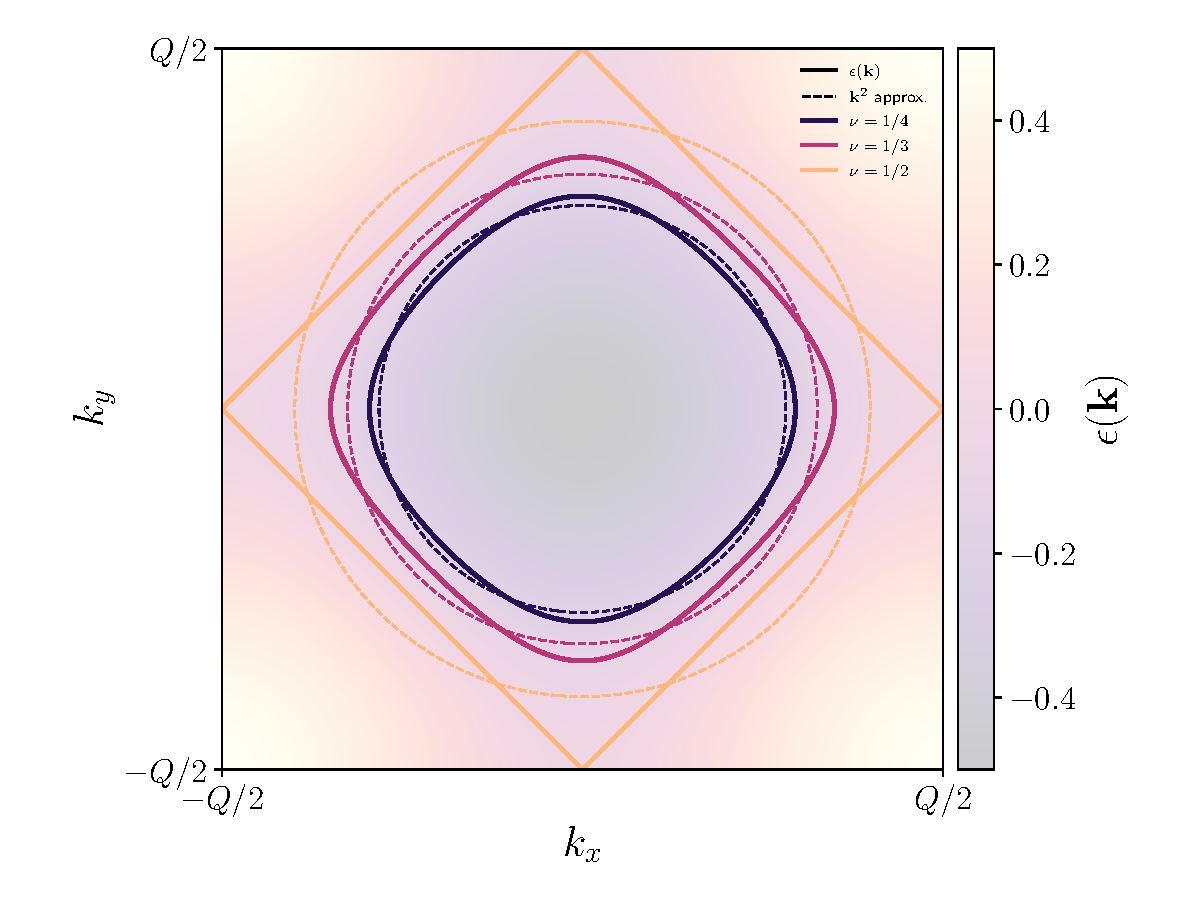
\includegraphics[width=0.6\textwidth]{plots/dispersion_with_fermi_surfaces_W_1.00.pdf}
    \caption{Dispersion $\varepsilon(\mathbf{k})$ at $W=1.0$, with the Fermi surfaces at fillings $\nu = 1/4, 1/3, 1/2$ shown both for the actual (cosine) dispersion and for a parabolic approximation.}\label{fig:fermi_surface}
\end{figure}

As shown in Fig.~\ref{fig:fermi_surface}, the Fermi surface (and even more so the density of states) of the actual dispersion differs significantly from that of the parabolic approximation, especially near the Van Hove singularity approached at $\nu = \tfrac{1}{2}$. We therefore relax this assumption: a similar criterion is derived below in which the Fermi surface is still taken to be circular for simplicity, but the density of states is obtained by numerically integrating the actual dispersion rather than assumed in a closed form.

Here $W$ is assumed to be large enough that the occupation follows a Fermi--Dirac step, $n_\tau(\mathbf{k}) = \theta(k_{F\tau}- |\mathbf{k}|)$ with $k_{F\tau}=\sqrt{2\nu_\tau}$. % chktex 8

\paragraph{Hartree energy ($\alpha=0$).} Since $\tilde U_{\tau\tau'}(0)=2\pi d_{\text{SC}}$ is independent of valley at $\alpha=0$,
\begin{equation}
    \langle \hat{H}_H \rangle = \frac{2\pi d_{\text{SC}}}{A} \sum_{\mathbf{k}, \mathbf{k'}} \sum_{\tau, \tau'} \langle n_{\mathbf{k},\tau} \rangle \langle n_{\mathbf{k'},\tau'} \rangle = \frac{2\pi d_{\text{SC}} N_{\phi}^2}{A} {(\nu_+ + \nu_-)}^2,
    \label{eq:hartree_energy_w}
\end{equation}
independent of the valley polarization.

\paragraph{Exchange energy.} At $\alpha=0$, $\tilde U_{\tau\tau}(\mathbf q) = u_0(\mathbf q)$, giving
\begin{equation}
    \langle \hat{H}_X \rangle = -\frac{1}{A} \sum_{\mathbf{q}} u_0(\mathbf{q}) e^{-q^2/2} \sum_{\tau, \mathbf{k}} n_\tau(\mathbf{k+q}) \, n_\tau(\mathbf{k}).
    \label{eq:exchange_energy_start}
\end{equation}
Converting sums to integrals ($\sum_{\mathbf{k}} \to \frac{A}{{(2\pi)}^2}\int d^2k$, and similarly for $\mathbf q$),
\begin{equation}
    E_X = -\frac{A}{{(2\pi)}^4} \int d^2q\, u_0(\mathbf{q}) e^{-q^2/2} \sum_{\tau} \int d^2k\, \theta(k_{F\tau}-|\mathbf{k+q}|)\theta(k_{F\tau}-|\mathbf{k}|).
    \label{eq:exchange_energy_integral}
\end{equation}
The inner integral is exactly the overlap area of two disks of radius $k_{F\tau}$ with centers separated by $q$,
\begin{equation}
    F(k_{F\tau}, q) = 2 k_{F\tau}^2 \arccos\!\left(\frac{q}{2 k_{F\tau}}\right) - \frac{q}{2} \sqrt{4 k_{F\tau}^2 - q^2},
    \label{eq:overlap_area}
\end{equation}
so that
\begin{equation}
    E_X = -\frac{A}{{(2\pi)}^2} \int \frac{d^2q}{{(2\pi)}^2}\, u_0(\mathbf{q}) e^{-q^2/2} \sum_\tau F(k_{F\tau}, q).
    \label{eq:exchange_energy_grouped}
\end{equation}

\paragraph{Expansion around the unpolarized point.} Write $\nu_\tau = \nu + \tau\delta$, so that $\delta$ is the polarization ($\delta=0$ corresponds to the unpolarized state), and $k_{F\tau} =\sqrt{2\nu_{\tau}}$, approximating the Fermi surface as a circle. Expanding $F$ to second order in $\delta$ and integrating over angle,
\begin{equation}
    \left. \frac{d^2 E_X}{d \delta^2} \right|_{\delta=0} = -\frac{4A}{\nu} \int_0^{\sqrt{8\nu}} \frac{q \tanh(qd_{\text{SC}})\, e^{-q^2/2}}{{(2\pi)}^2 (1+l_{\text{RK}} q)\sqrt{8\nu - q^2}}\, dq \;\equiv\; -\frac{4A}{\nu}\, \mathcal{I}_2(\nu, d_{\text{SC}}).
    \label{eq:exchange_curvature}
\end{equation}
The kinetic-energy curvature follows directly from the dispersion, obtained numerically via the density of states $D(\nu)=d\mu/d\nu$ computed from $\varepsilon_\tau(\mathbf{k})$:
\begin{equation}
    \left. \frac{d^2 E_K}{d \delta^2} \right|_{\delta=0} = 2 A W \frac{d\mu}{d\nu} = \frac{A W}{\pi} D(\nu).
    \label{eq:kinetic_curvature}
\end{equation}
The transition occurs where the curvature of the unpolarized state changes sign, i.e.\ where the kinetic cost of polarizing exactly cancels the exchange gain:
\begin{equation}
    \left. \frac{d^2 E_K}{d\delta^2} \right|_{\delta=0} + \left. \frac{d^2 E_X}{d\delta^2} \right|_{\delta=0} = 0
    \quad\Longrightarrow\quad
    \frac{AW_c}{\pi} D(\nu) = \frac{4A}{\nu}\,\mathcal{I}_2(\nu, d_{\text{SC}}),
    \label{eq:wc_condition}
\end{equation}
giving
\begin{equation}
    W_c(\nu, d_{\text{SC}}) = \frac{4\pi\, \mathcal{I}_2(\nu, d_{\text{SC}})}{\nu\, D(\nu)}.
    \label{eq:wc_formula}
\end{equation}
This result extends straightforwardly to nonzero $\alpha$ via the same procedure, giving
\begin{equation}
    W_c(\nu, d_{\text{SC}}, \alpha) = \frac{4\pi\, (1+\alpha) \mathcal{I}_2(\nu, d_{\text{SC}})}{\nu\, D(\nu)}  - \frac{4\, \alpha d_{\text{SC}}}{D(\nu)}.
    \label{eq:wc_formula_alpha}
\end{equation}

\subsection{Comparison with the numerical mean-field estimates}

We evaluate the analytic estimates of Secs.~\ref{subsec:alpha_transition}--\ref{subsec:w_transition} numerically at the default parameters $d_{\text{SC}}=6a$, $l_{\text{RK}}=0$, using $D(\nu)$ obtained from the actual cosine dispersion (Fig.~\ref{fig:fermi_surface}) rather than the parabolic approximation, and compare against the ED phase diagrams below.

At $W=0$, Eqs.~\eqref{eq:alpha_c_case1}--\eqref{eq:alpha_c_case2} give $\alpha_c \approx 0.042$ at $\nu=\frac13$ per valley, compared to the ED value $\alpha_c \approx 0.004$ extracted from Fig.~\ref{fig:third_third_phase_diagram}. The mean-field estimate thus overestimates $\alpha_c$ by roughly an order of magnitude, but correctly predicts the direction of the polarized phase ($\alpha < \alpha_c$ in the $U(\mathbf{q}=0)\neq 0$ case), proximity to the valley-isotropic point and, more importantly, its trend: scanning $\alpha_c(d_{\text{SC}})$ and $\alpha_c(l_{\text{RK}})$ analytically gives a monotonic decrease with both parameters, matching the monotonic narrowing of the $\alpha$-stable FQH region with increasing $d_{\text{SC}}$ and $l_{\text{RK}}$ observed in Figs.~\ref{fig:third_third_screening_alpha_vs_d_phase_diagram_a} and~\ref{fig:third_third_screening_alpha_vs_lRK_phase_diagram_b}.


For the $W$-driven depolarization transition, the mean-field estimate at $\nu = \tfrac13$, $\alpha = 0$ gives $W_c \approx 0.84$, compared to the ED result of $W \sim 0.5$ read off from Fig.~\ref{fig:third_third_phase_diagram}. As with $\alpha_c$, the analytic estimate is systematically too large but of the correct order of magnitude, consistent with the general tendency of Hartree-Fock to overestimate the stability of ordered phases by neglecting quantum fluctuations.


Overall, the analytic mean-field treatment reproduces the correct qualitative structure of the phase diagram --- the existence and approximate location of both the $\alpha$- and $W$-driven depolarization transitions, and their correct monotonic dependence on the screening parameters $d_{\text{SC}}$ and $l_{\text{RK}}$ --- while systematically overestimating both $\alpha_c$ and $W_c$.

\section{\texorpdfstring{Phase diagram for $\nu = \frac{2}{3}$}{Phase diagram for nu = 2/3}}\label{sec:third_third_results}

At this filling, an FQH state is expected at $W=0$ in the valley-polarized region, and an FTI state at $\alpha=1$, $W=0$. We now present the numerical phase diagram, addressing how resilient these topological phases are against nonzero $|W|$ and non-ideal $\alpha$, and examine phase transitions found in the system, and the dependence of stability of topological phases on the screening parameters $d_{\text{SC}}$ and $l_{\text{RK}}$.

\begin{figure}[htbp]
    \centering
    \begin{subfigure}{0.45\textwidth}
        \centering
        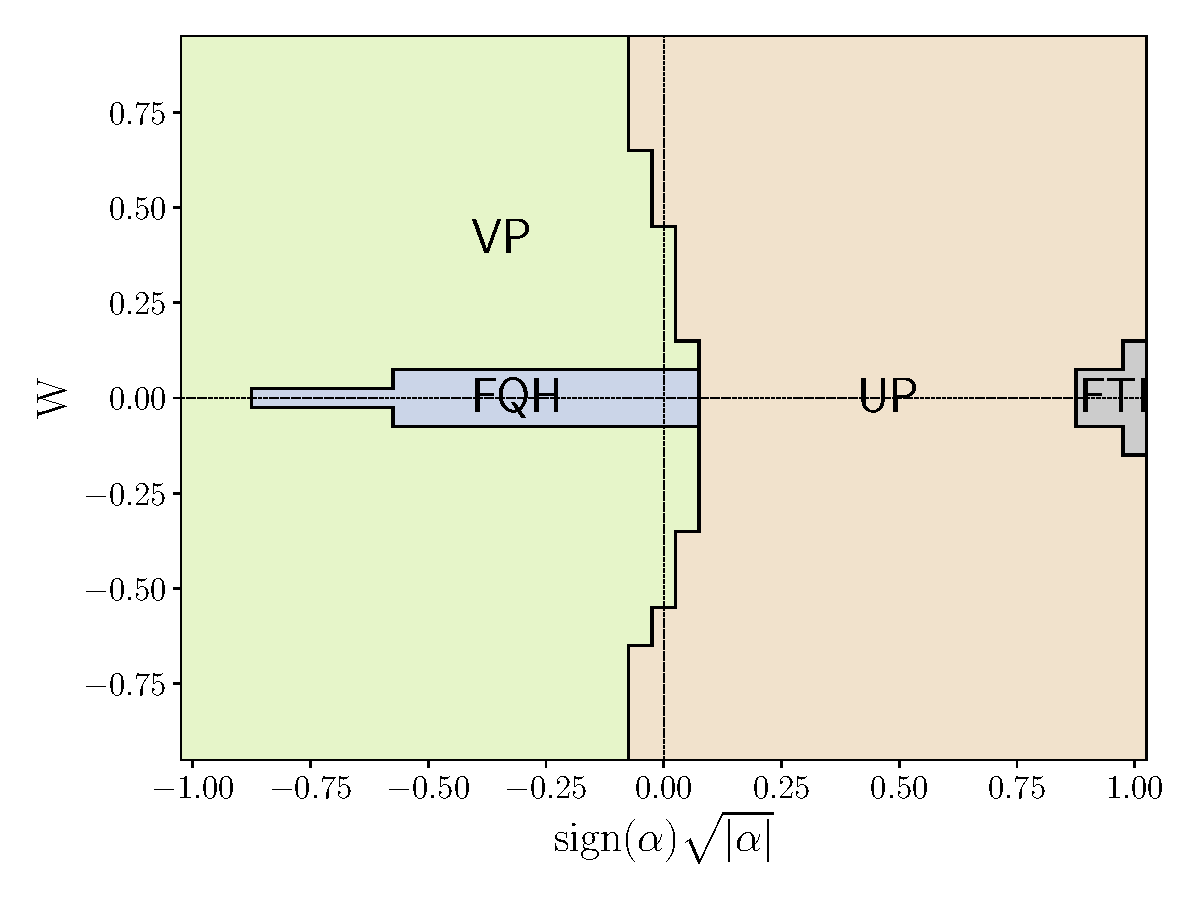
\includegraphics[width=1.0\textwidth]{plots/third_third_phase_diagram.pdf}
        \subcaption{$U(\mathbf{q}=0) \neq 0$}\label{fig:third_third_phase_diagram}
    \end{subfigure}
    \begin{subfigure}{0.45\textwidth}
        \centering
        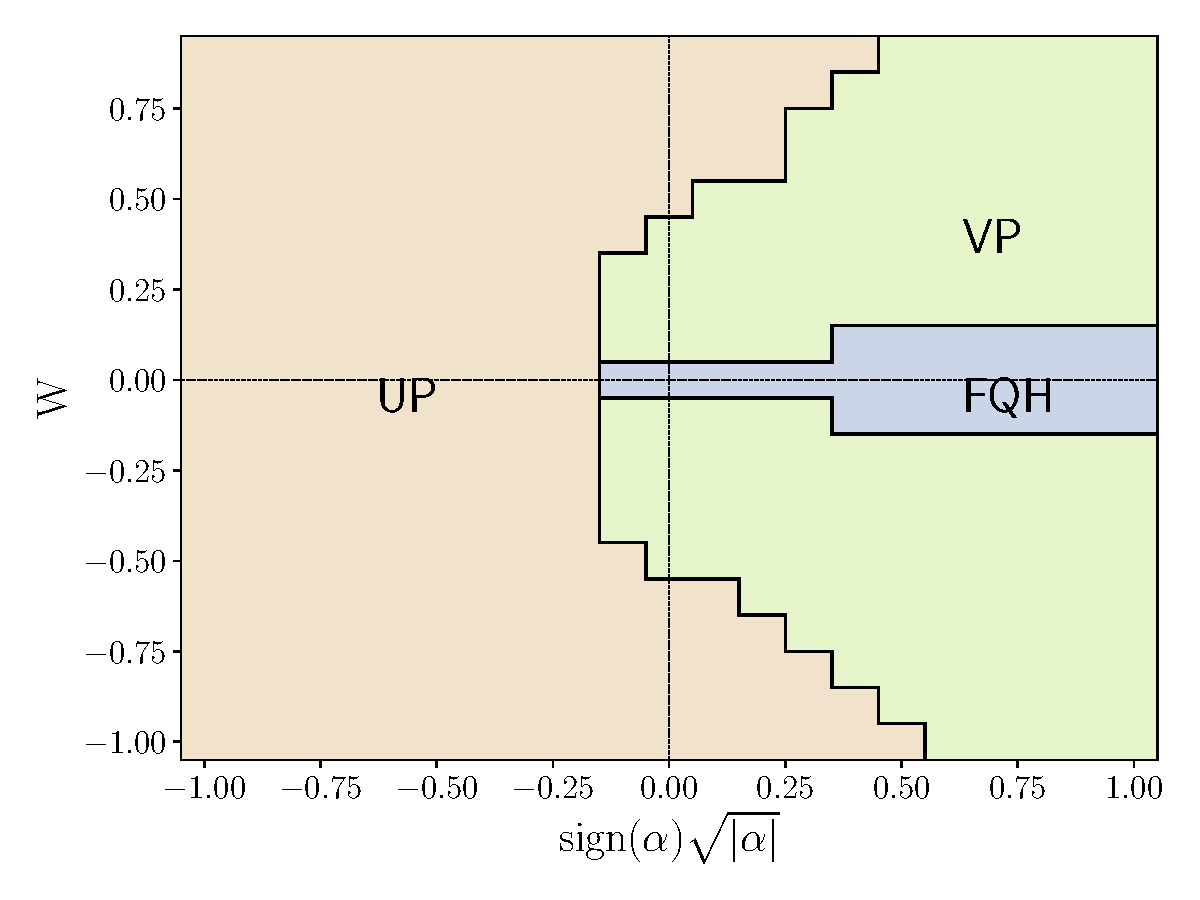
\includegraphics[width=1.0\textwidth]{plots/third_third_q0_phase_diagram.pdf}
        \subcaption{$U(\mathbf{q}=0) = 0$}\label{fig:third_third_q0_phase_diagram}
    \end{subfigure}
    \begin{subfigure}{0.45\textwidth}
        \centering
        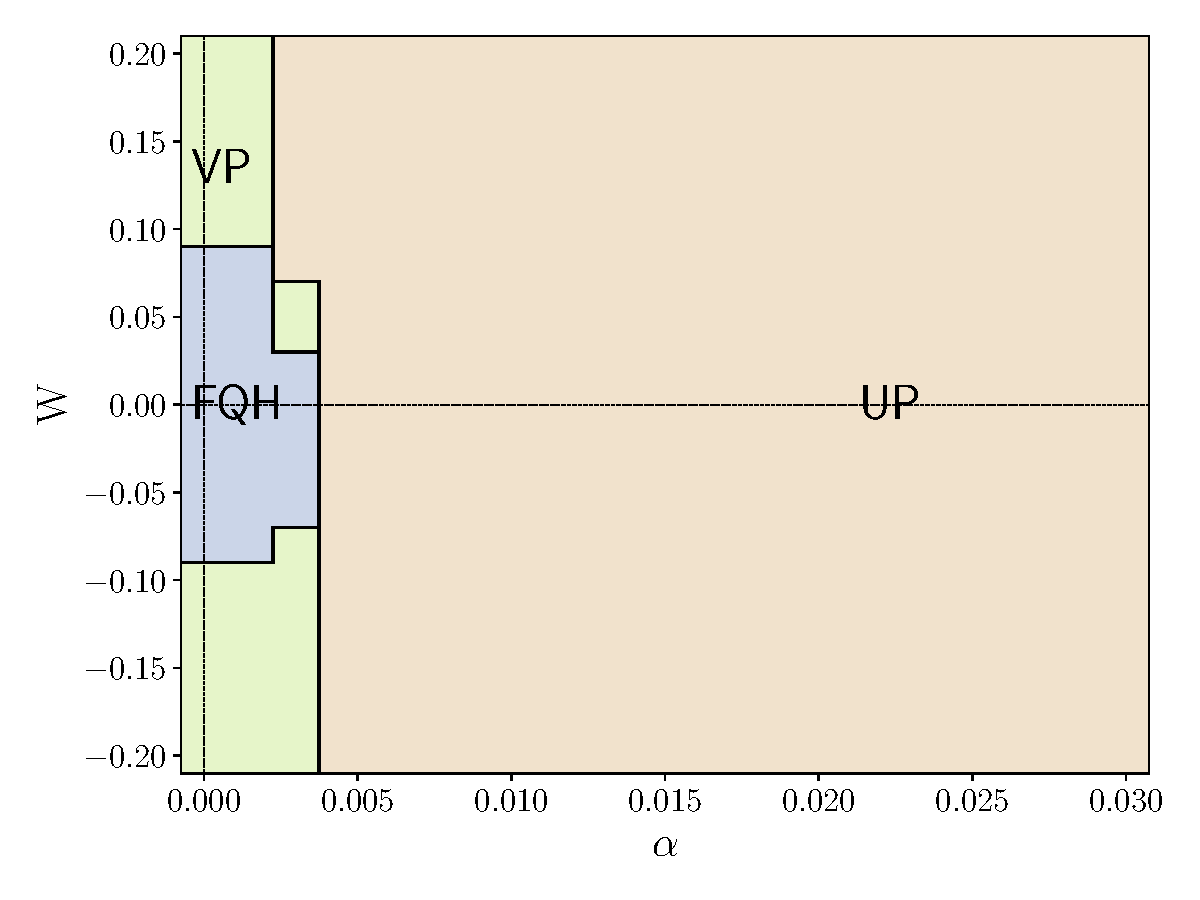
\includegraphics[width=1.0\textwidth]{plots/third_third_zoom_3_phase_diagram.pdf}
        \subcaption{Zoom-in on the FQH ($U(\mathbf{q}=0) \neq 0$)}\label{fig:third_third_zoom_3_phase_diagram}
    \end{subfigure}
    \begin{subfigure}{0.45\textwidth}
        \centering
        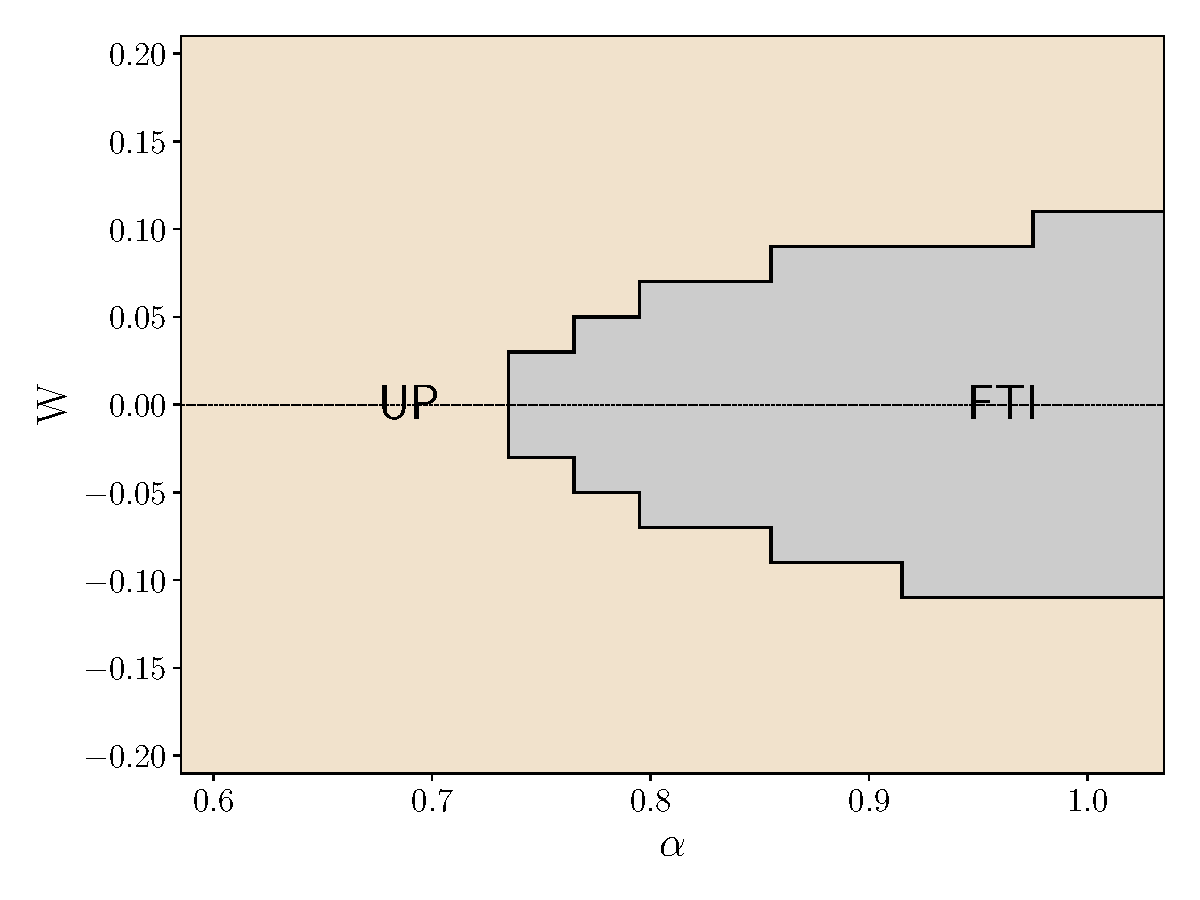
\includegraphics[width=1.0\textwidth]{plots/third_third_zoom_9_phase_diagram.pdf}
        \subcaption{Zoom-in on the FTI ($U(\mathbf{q}=0) \neq 0$)}\label{fig:third_third_zoom_9_phase_diagram}
    \end{subfigure}
    \caption{Phase diagrams of the $\nu = \frac{2}{3}$ filling. VP:\@ gapless valley-polarized state. UP:\@ general unpolarized state. FQH:\@ 3-fold degenerate valley-polarized fractional quantum Hall state. FTI:\@ 9-fold degenerate valley-unpolarized fractional topological insulator. See Fig.~\ref{fig:summary} for a schematic identification of the UP regions.}\label{fig:third_third_phases}
\end{figure}

Figure~\ref{fig:third_third_phases} presents the phase diagram at $\nu=\frac{2}{3}$. The only significant gaps found in the system are $\Delta_3$, $\Delta_6$ (discussed below) and $\Delta_9$. In the $U(\mathbf{q}=0) \neq 0$ case (Fig.~\ref{fig:third_third_phase_diagram}), full valley polarization is observed at low $|W|$ and low $\alpha$, with $\alpha_c \approx 0.004$, while the unpolarized state prevails at larger $\alpha$. At $\alpha=1$, down to $\alpha \approx 0.72$, the unpolarized state shows a clear 9-fold degeneracy, consistent with the FTI state (each FQH copy contributing a 3-fold degeneracy). The valley-polarized region itself splits into two parts. At low $|W|$ the state has a topological 3-fold degeneracy, consistent with a $\nu=\frac{2}{3}$ FQH state in a single valley. The topological nature of FQH and FTI phases is confirmed below via spectral flow. Both of them survive a nonzero bandwidth, up to $|W| \approx 0.09$ for the FQH state and $|W| \approx 0.1$ for the FTI state. The similarity of these two values is consistent with the ideal FQH and FTI states incurring the same kinetic energy penalty from $W$. At intermediate $|W|$, the FQH state transitions into a gapless valley-polarized state (denoted as VP) --- driven by the kinetic-energy cost of the flat momentum occupation characteristic of the FQH state --- and, at an $\alpha$-dependent $W_c$ on the order of $\pm0.5$, into a valley-unpolarized state. The FTI state undergoes an analogous transition into a gapless state at increasing $W$.

The phase diagram is approximately symmetric about the $W=0$ axis, as suspected from the analysis in \S\ref{sec:symmetries}. The symmetry being only approximate is a finite size effect, in particular related to the fact that the sampling of the Brillouin zone is not invariant under the $\pm \mathbf{Q_0}$ shift. At $\alpha \to -1$, the FQH state is not detected, since valley polarization combined with the vanishing intra-valley interaction renders the system effectively noninteracting, closing the spectral gap.

A different picture emerges for the $U(\mathbf{q}=0) = 0$ phase diagram (Fig.~\ref{fig:third_third_q0_phase_diagram}), where the valley-polarized region instead occupies large $\alpha$, and the unpolarized --- small $\alpha$. The same VP and FQH phases appear, with a similar $W$-dependent transition between them, but because the polarized phase now extends across the entire $\alpha > 0$ region, no FTI state is found. At low $\alpha$, only a non-polarized gapless state is found --- it is not investigated further.

\subsection{\texorpdfstring{Phase transitions at $W\approx0$ and variable $\alpha$}{Phase transitions at W approx 0 and variable alpha}}

\begin{figure}[htbp]
    \centering
    \begin{subfigure}{0.3\textwidth}
        \centering
        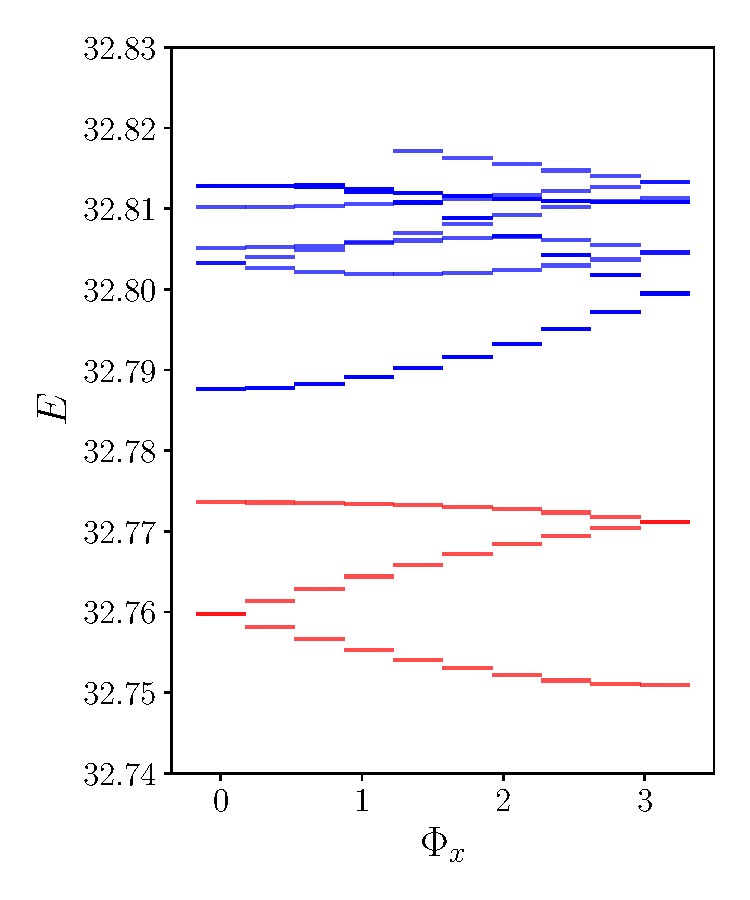
\includegraphics[width=1.0\textwidth]{plots/alpha_transition_W=0.05_alpha=0.0024.pdf}
        \subcaption{$\alpha = 0.0024$ --- FQH}\label{fig:low_alpha_transition_a}
    \end{subfigure}
    \begin{subfigure}{0.3\textwidth}
        \centering
        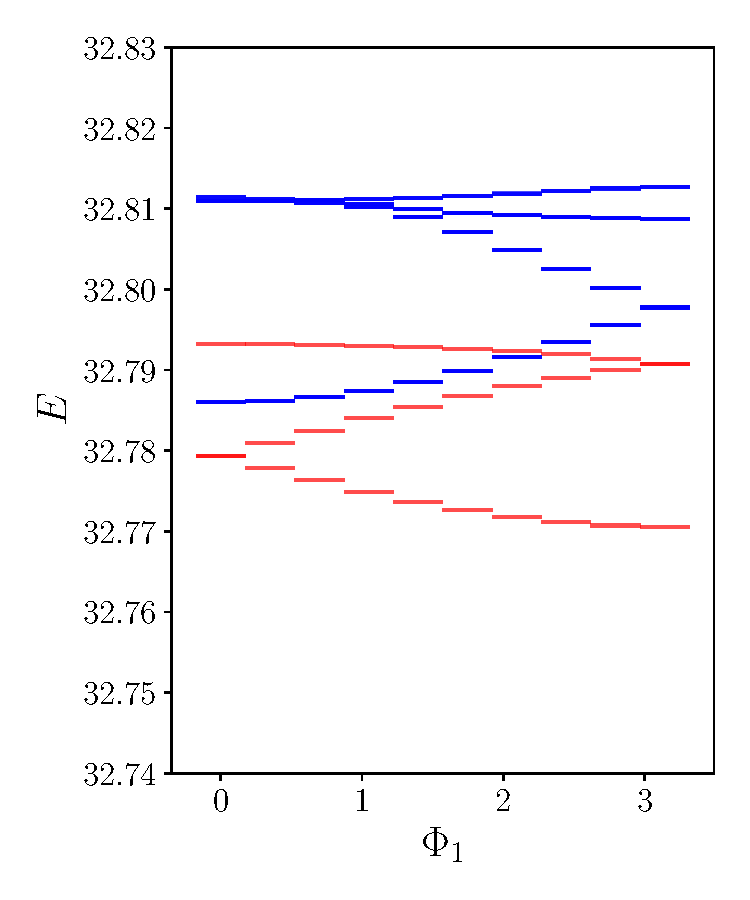
\includegraphics[width=1.0\textwidth]{plots/alpha_transition_W=0.05_alpha=0.003.pdf}
        \subcaption{$\alpha = 0.003$ --- gapless}\label{fig:low_alpha_transition_b}
    \end{subfigure}
    \begin{subfigure}{0.3\textwidth}
        \centering
        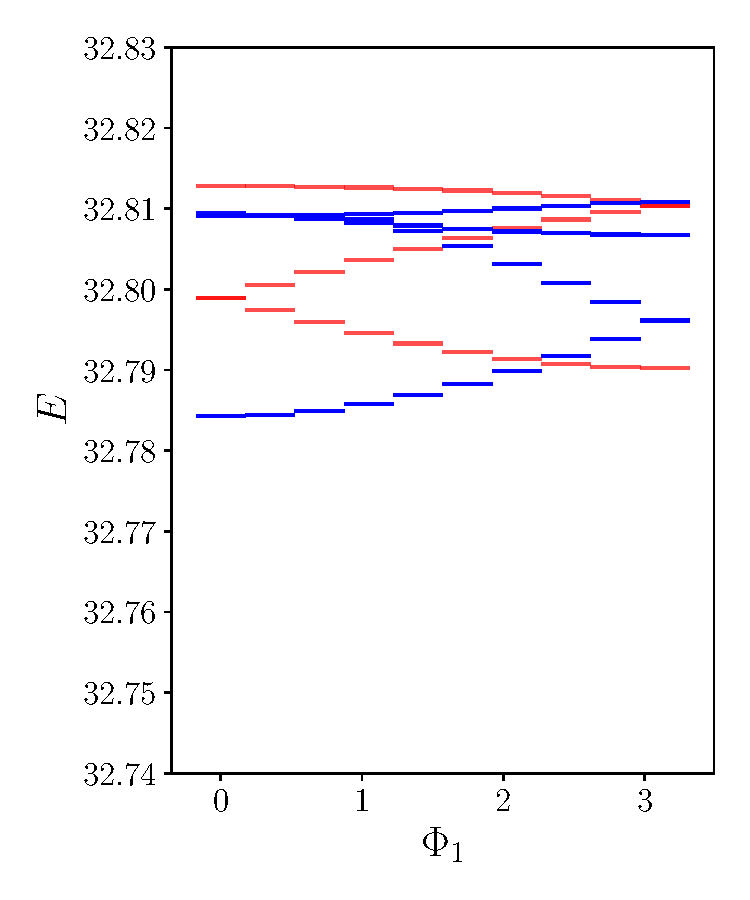
\includegraphics[width=1.0\textwidth]{plots/alpha_transition_W=0.05_alpha=0.0036.pdf}
        \subcaption{$\alpha = 0.0036$ --- gapless}\label{fig:low_alpha_transition_c}
    \end{subfigure}
    \caption{Flux insertion plots of the energy spectrum near the valley-isotropic limit $\alpha\approx 0$, at $W=0.05$ and $\nu = \frac{2}{3}$, showing the transition from the FQH state to a gapless state. Ground-state manifold shown in red.}\label{fig:low_alpha_transition}
\end{figure}

The nature of the phase transition out of the FQH state is illustrated in Figure~\ref{fig:low_alpha_transition}, which shows the energy spectrum under flux insertion at $W=0.05$ for different $\alpha$ values, across the transition out of the FQH phase. Interestingly, the 3-fold degenerate ground-state manifold survives the transition; the only change is the relative energy of the manifold with respect to the gapless continuum above it.

\begin{figure}[htbp]
    \centering
    \begin{subfigure}{0.3\textwidth}
        \centering
        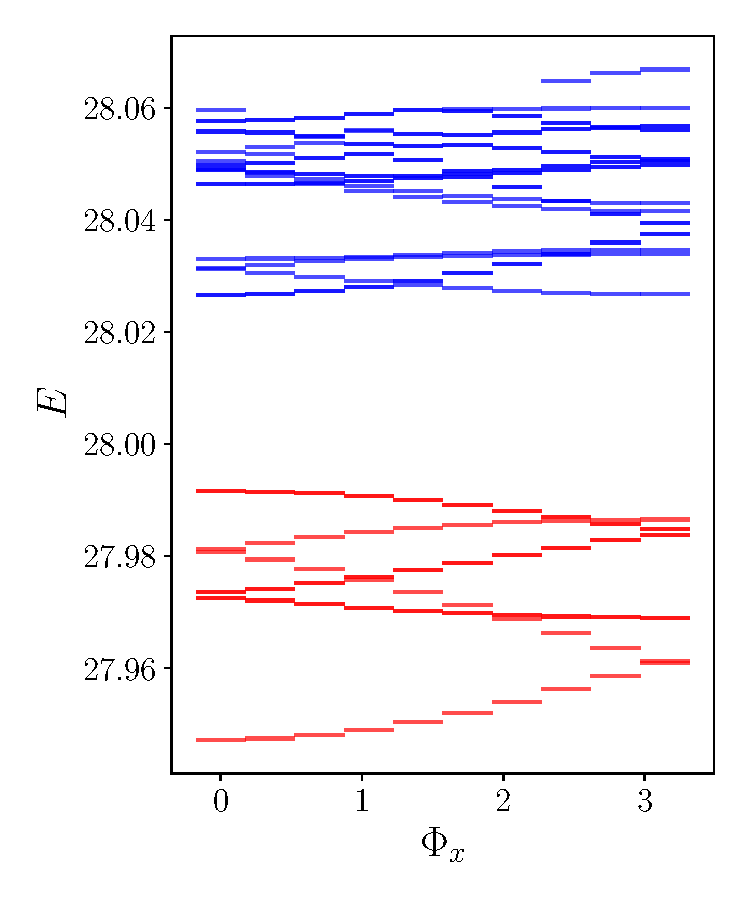
\includegraphics[width=1.0\textwidth]{plots/alpha1_transition_W=0.05_alpha=0.8500000000000001.pdf}
        \subcaption{$\alpha = 0.85$ --- FTI state}\label{fig:high_alpha_transition_a}
    \end{subfigure}
    \begin{subfigure}{0.3\textwidth}
        \centering
        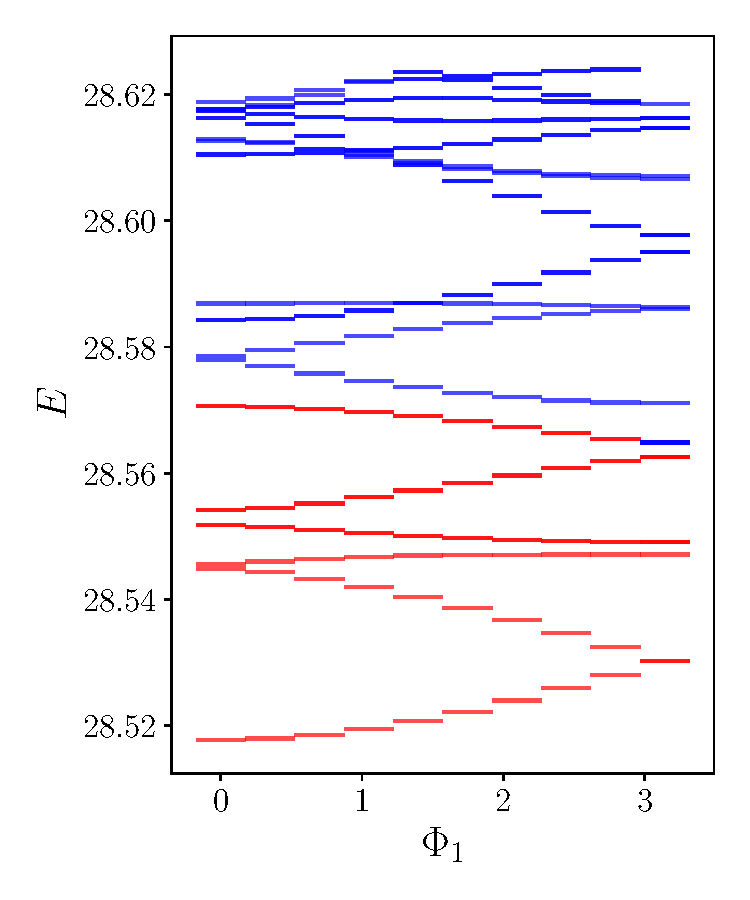
\includegraphics[width=1.0\textwidth]{plots/alpha1_transition_W=0.05_alpha=0.76.pdf}
        \subcaption{$\alpha = 0.76$ --- gapless state}\label{fig:high_alpha_transition_b}
    \end{subfigure}
    \caption{Phase winding of the energy spectrum near the decoupled limit $\alpha \approx 1$, at $W=0.05$ and $\nu = \frac{2}{3}$, showing the transition from the FTI state to a gapless state. Ground-state manifold shown in red.}\label{fig:high_alpha_transition}
\end{figure}

Figure~\ref{fig:high_alpha_transition} shows the analogous phase winding at $W=0.05$ with $\alpha$ decreasing from the FTI-like state. As before, the ground-state manifold moves relative to the excited-state continuum until the 9-fold degenerate gap closes. However, the relative energy splitting between the lowest 3 states of the ground-state manifold and the remaining 6 grows on approach to the transition, eventually opening a gap between them: a nonzero 3-fold gap in the otherwise unpolarized state is indeed found in a small region of the phase diagram. As described below (\S\ref{sec:third_third_density}), this phase is not topological.

\subsection{\texorpdfstring{Spectral flow \& phase transitions with variable $W$}{Phase transitions with variable W}}

\begin{figure}[htbp]
    \centering
    \begin{subfigure}{0.3\textwidth}
        \centering
        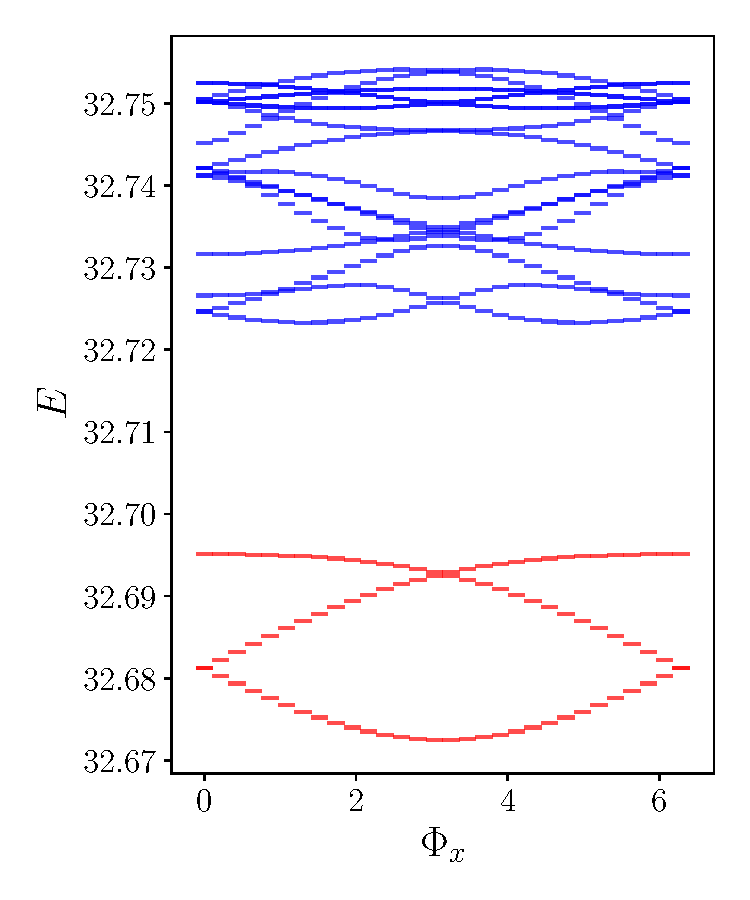
\includegraphics[width=1.0\textwidth]{plots/phase_winding_W=0.05_alpha=0.0.pdf}
        \subcaption{$W=0.05$}\label{fig:phase_winding_low_alpha_a}
    \end{subfigure}
    \begin{subfigure}{0.3\textwidth}
        \centering
        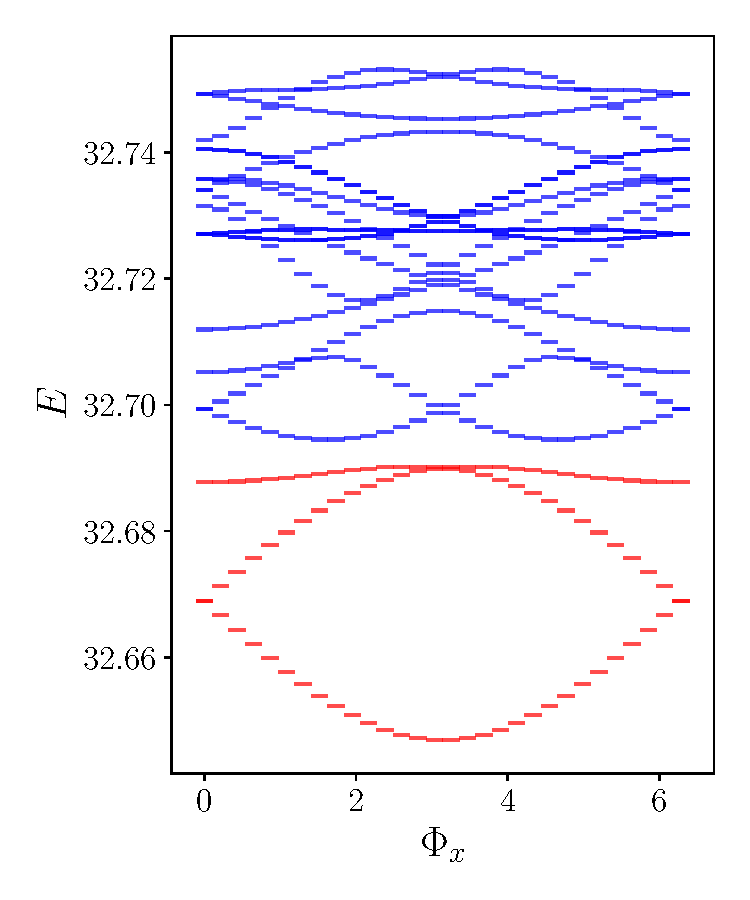
\includegraphics[width=1.0\textwidth]{plots/phase_winding_W=0.1_alpha=0.0.pdf}
        \subcaption{$W=0.1$}\label{fig:phase_winding_low_alpha_b}
    \end{subfigure}
    \begin{subfigure}{0.3\textwidth}
        \centering
        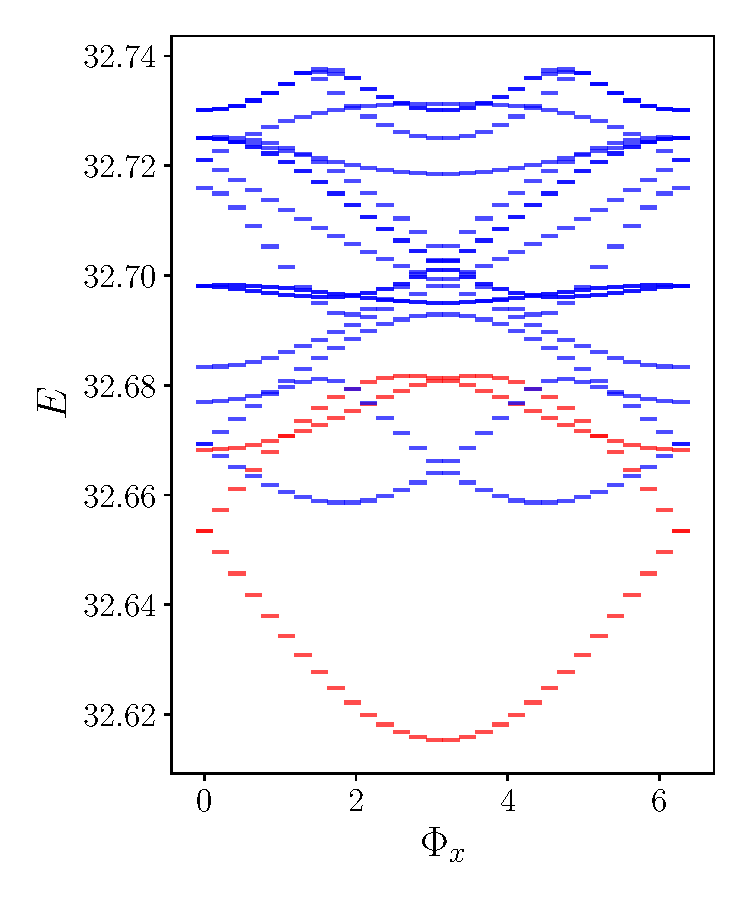
\includegraphics[width=1.0\textwidth]{plots/phase_winding_W=0.15_alpha=0.0.pdf}
        \subcaption{$W=0.15$}\label{fig:phase_winding_low_alpha_c}
    \end{subfigure}
    \caption{Phase winding of the energy spectrum at $\alpha=0$ and $\nu = \frac{2}{3}$, showing the transition from the FQH state to a gapless state with increasing $W$. Ground-state manifold shown in red.}\label{fig:phase_winding_low_alpha}
\end{figure}

\begin{figure}[htbp]
    \centering
    \begin{subfigure}{0.3\textwidth}
        \centering
        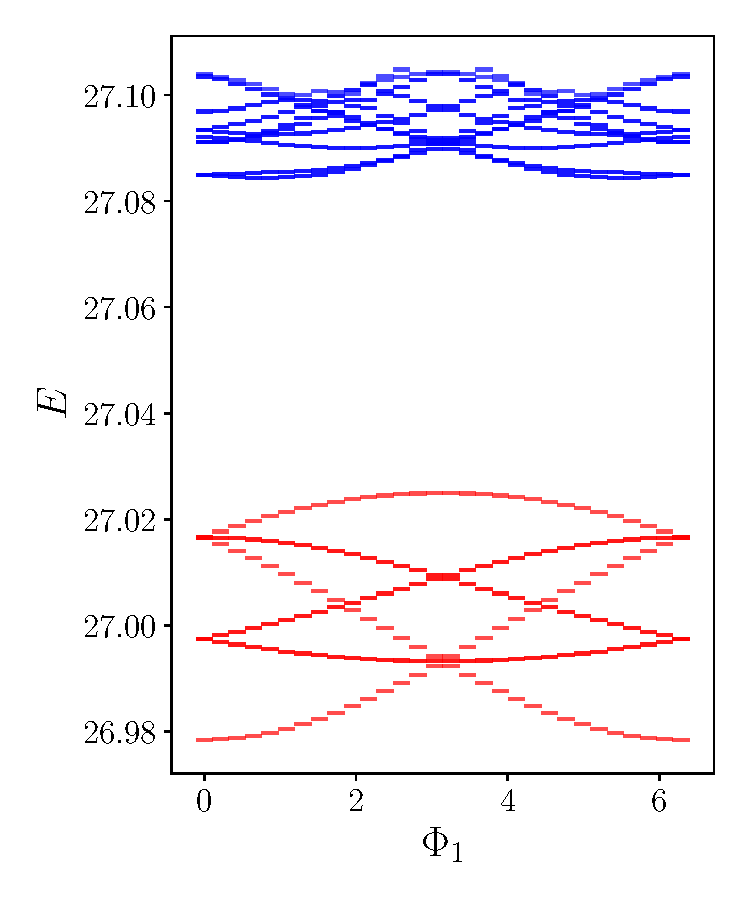
\includegraphics[width=1.0\textwidth]{plots/phase_winding_W=0.05_alpha=1.0.pdf}
        \subcaption{$W=0.05$}\label{fig:phase_winding_high_alpha_a}
    \end{subfigure}
    \begin{subfigure}{0.3\textwidth}
        \centering
        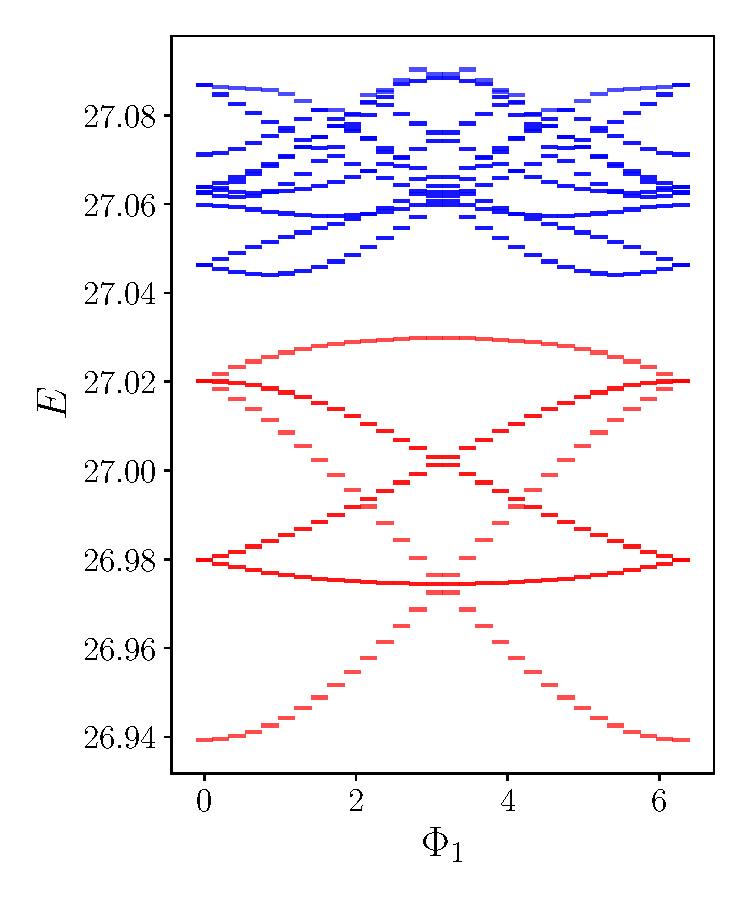
\includegraphics[width=1.0\textwidth]{plots/phase_winding_W=0.1_alpha=1.0.pdf}
        \subcaption{$W=0.1$}\label{fig:phase_winding_high_alpha_b}
    \end{subfigure}
    \begin{subfigure}{0.3\textwidth}
        \centering
        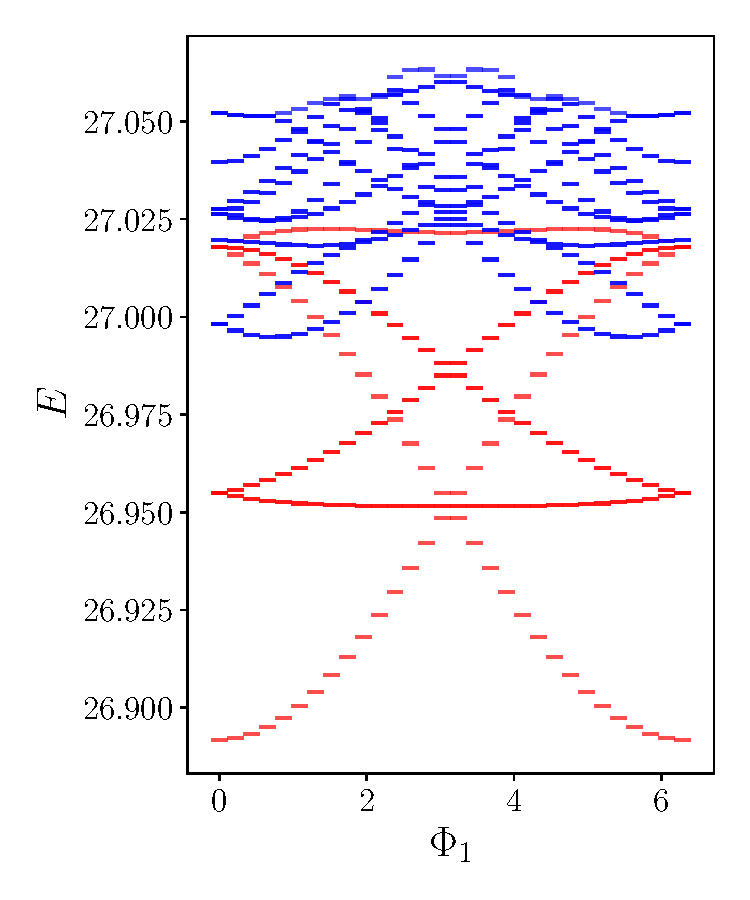
\includegraphics[width=1.0\textwidth]{plots/phase_winding_W=0.15_alpha=1.0.pdf}
        \subcaption{$W=0.15$}\label{fig:phase_winding_high_alpha_c}
    \end{subfigure}
    \caption{Phase winding of the energy spectrum at $\alpha=1$ and $\nu = \frac{2}{3}$, showing the transition from the FTI state to a gapless state with increasing $W$. Ground-state manifold shown in red.}\label{fig:phase_winding_high_alpha}
\end{figure}

Figures~\ref{fig:phase_winding_low_alpha} and~\ref{fig:phase_winding_high_alpha} show the energy spectrum for the FQH ($\alpha=0.0$) and FTI ($\alpha=1$) phases respectively, under flux insertion. At low $W$ (Figs.~\ref{fig:phase_winding_low_alpha_a} and~\ref{fig:phase_winding_high_alpha_a}), spectral flow of the ground-state manifold is directly observed: the spectrum at $\Phi_1 = 0$ and $\Phi_1 = 2\pi$ is identical, but the states within the manifold are cyclically permuted, returning to their original positions only after $\Phi_1 = 6\pi$. This further confirms the topological nature of both phases. The remaining panels of each figure visualize the transition from the topological to the gapless phase as the increasing bandwidth closes the spectral gap.

\subsection{\texorpdfstring{Nature of the intermediate--$\alpha$ and high-$|W|$ phases}{Nature of the intermediate-alpha and high-W phases}}\label{sec:third_third_density}

\begin{figure}[htbp]
    \centering
    \begin{subfigure}{0.45\textwidth}
        \centering
        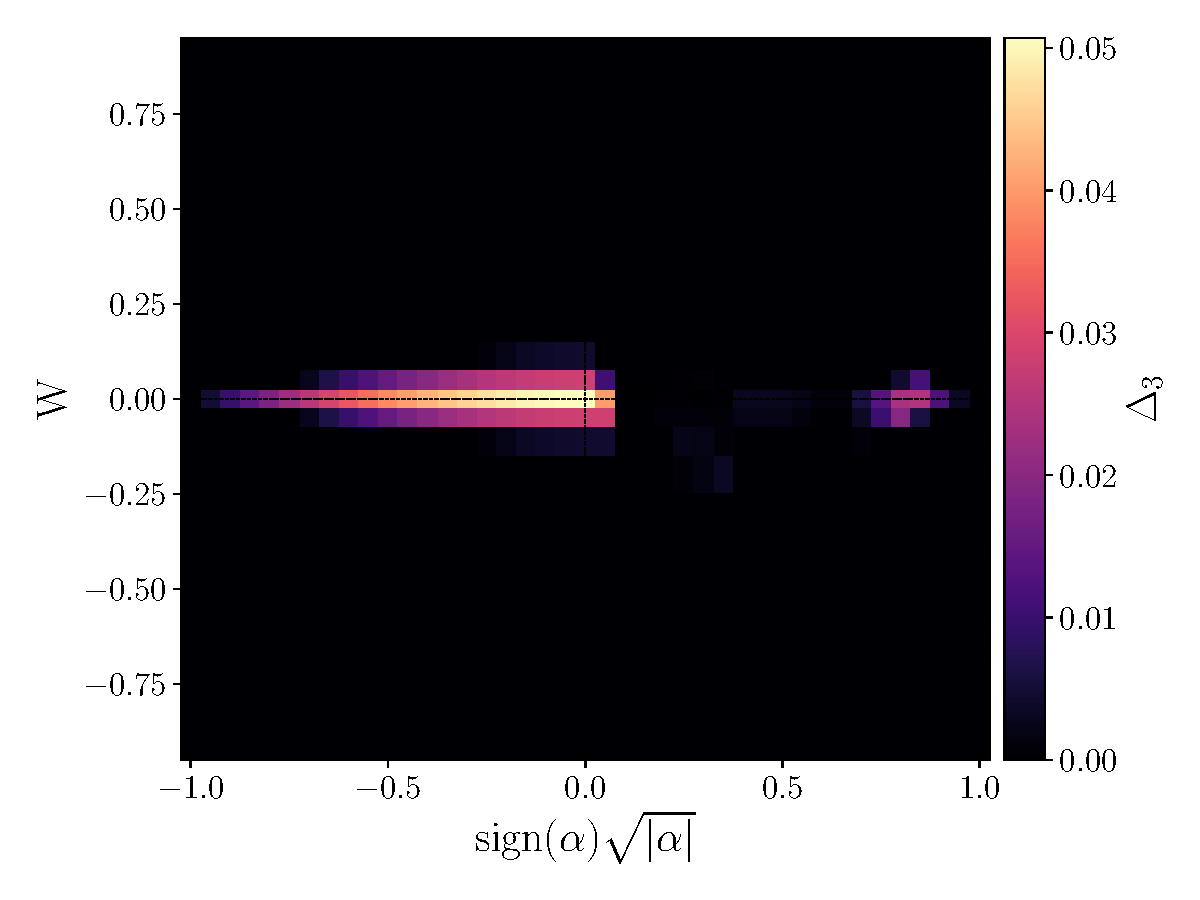
\includegraphics[width=1.0\textwidth]{plots/third_third_gap_n3.pdf}
        \subcaption{$\Delta_3$}\label{fig:third_third_gap_n3}
    \end{subfigure}
    \begin{subfigure}{0.45\textwidth}
        \centering
        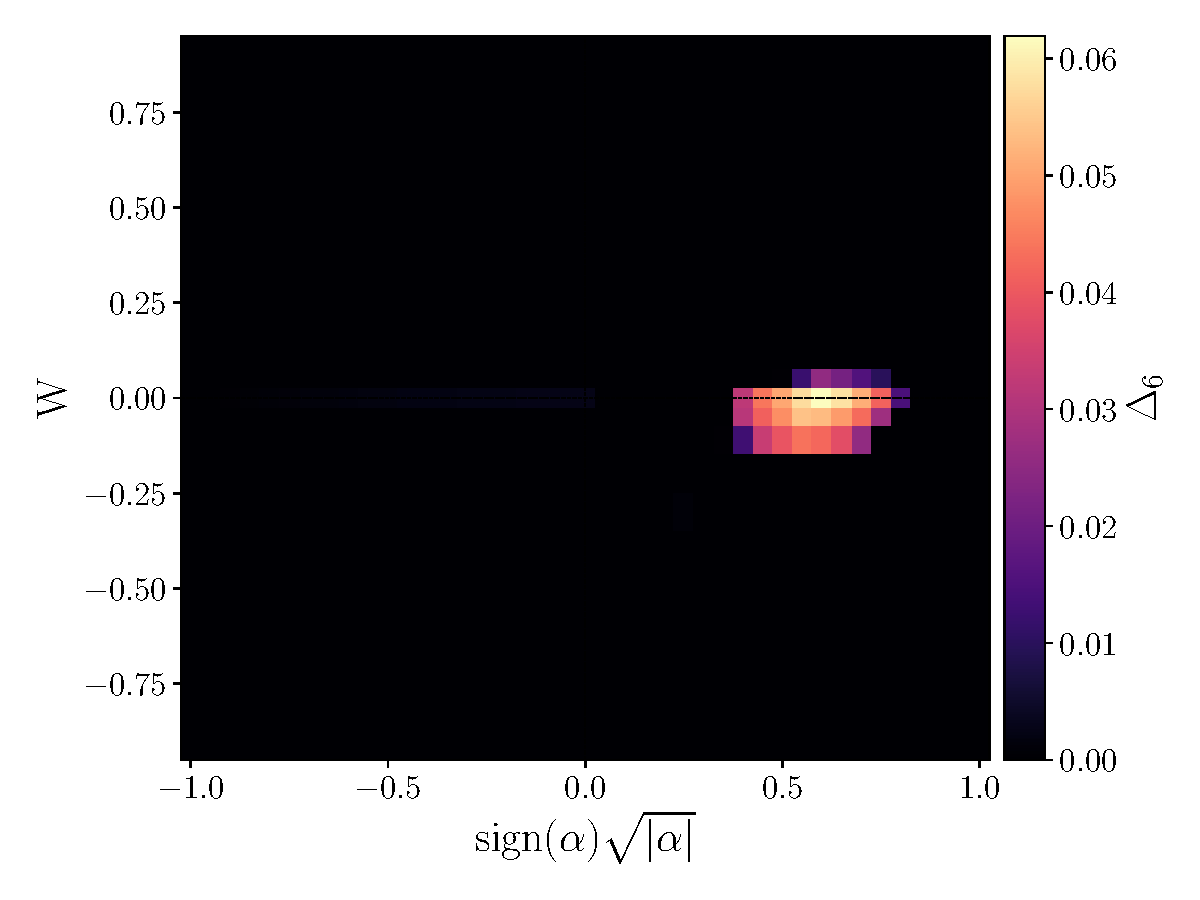
\includegraphics[width=1.0\textwidth]{plots/third_third_gap_n6.pdf}
        \subcaption{$\Delta_6$}\label{fig:third_third_gap_n6}
    \end{subfigure}
    \begin{subfigure}{0.45\textwidth}
        \centering
        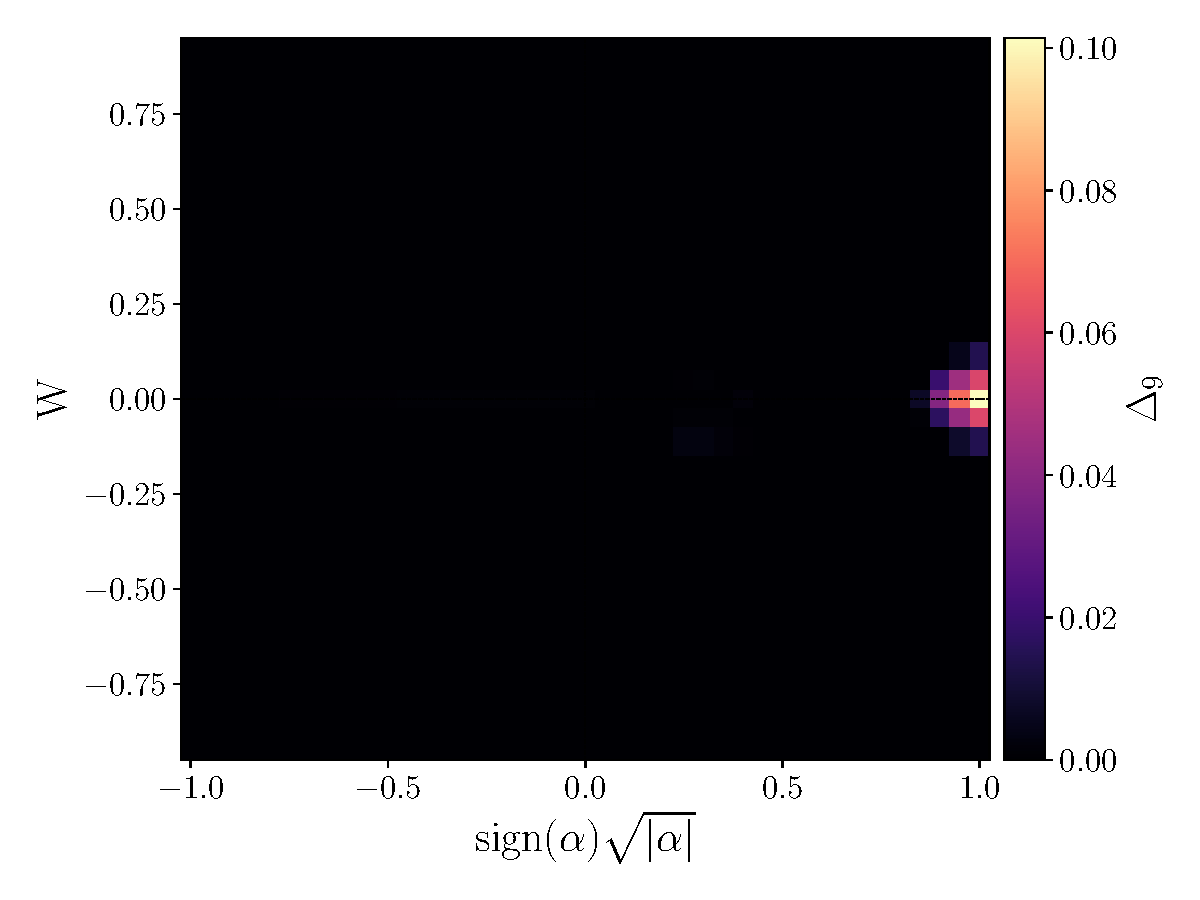
\includegraphics[width=1.0\textwidth]{plots/third_third_gap_n9.pdf}
        \subcaption{$\Delta_9$}\label{fig:third_third_gap_n9}
    \end{subfigure}
    \begin{subfigure}{0.25\textwidth}
        \centering
        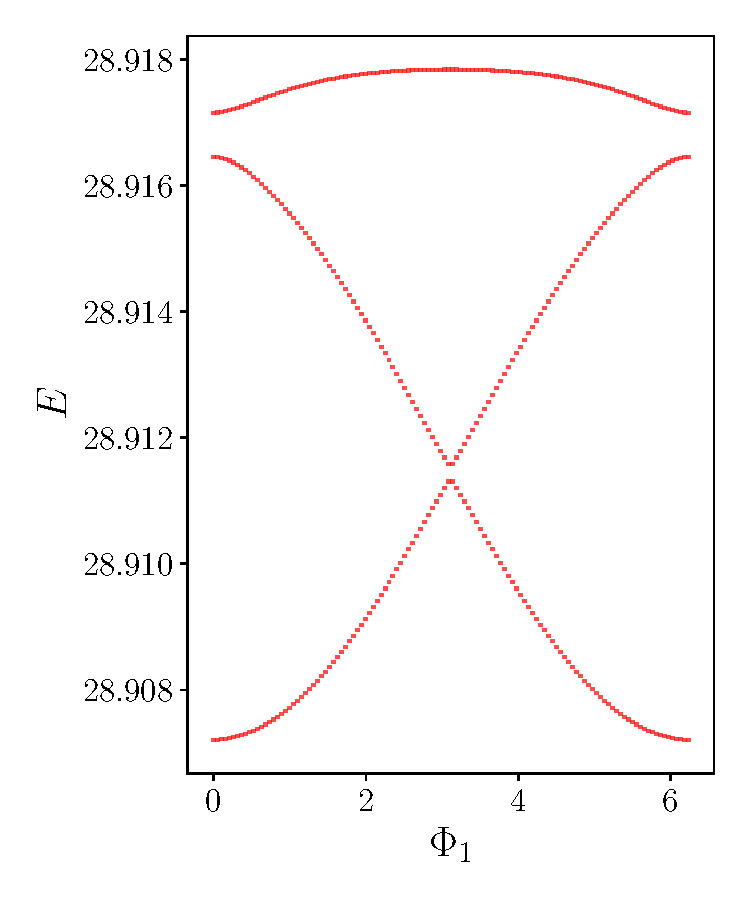
\includegraphics[width=1.0\textwidth]{plots/phase_winding_halperin_W=0.025_alpha=0.7.pdf}
        \subcaption{$\alpha=0.7$, $W=0.025$}\label{fig:phase_winding_3fold_degenerate}
    \end{subfigure}
    \begin{subfigure}{0.25\textwidth}
        \centering
        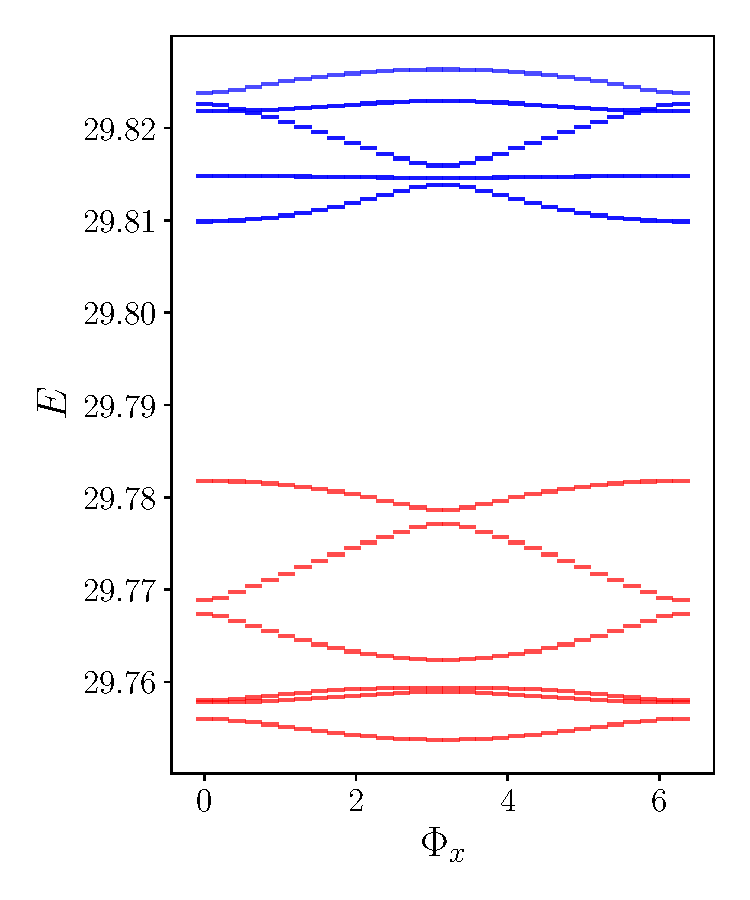
\includegraphics[width=1.0\textwidth]{plots/phase_winding_W=0.025_alpha=0.5625.pdf}
        \subcaption{$\alpha=0.56$, $W=0.025$}\label{fig:phase_winding_6fold_degenerate}
    \end{subfigure}
    \caption{(a-c) Spectral gaps in the system as a function of $\alpha$ and $W$, at $\nu=\frac{2}{3}$. (d-e) Flux insertion of the 3-fold and 6-fold degenerate states, respectively.}\label{fig:third_third_gaps}
\end{figure}

Figure~\ref{fig:third_third_gaps} shows the size of the $\Delta_3$, $\Delta_6$, and $\Delta_9$ gaps across the phase diagram. It confirms directly that the FQH and FTI states are most stable at $W=0$, where the corresponding gap is largest. Notably, non-zero $\Delta_3$ and $\Delta_6$ gaps are also found in the unpolarized phase at intermediate $\alpha$. However, as shown in Fig.~\ref{fig:phase_winding_6fold_degenerate}~and~\ref{fig:phase_winding_3fold_degenerate}, both the 3-fold and the 6-fold degenerate states do not exhibit spectral flow --- the energy levels do not cross or permute --- and are therefore not topological. It could correspond to a charge-density-wave state or be an artifact of a finite system size. Because of their uncertain nature and small extent, they were not investigated further and are included under the umbrella ``UP'' region of the phase diagram.

To further examine the UP region and the assumptions underlying the mean-field treatment of Sec.~\ref{sec:meanfield}, the momentum-occupation function $n(\mathbf{k})$ is also calculated.

\begin{figure}[htbp]
    \centering
    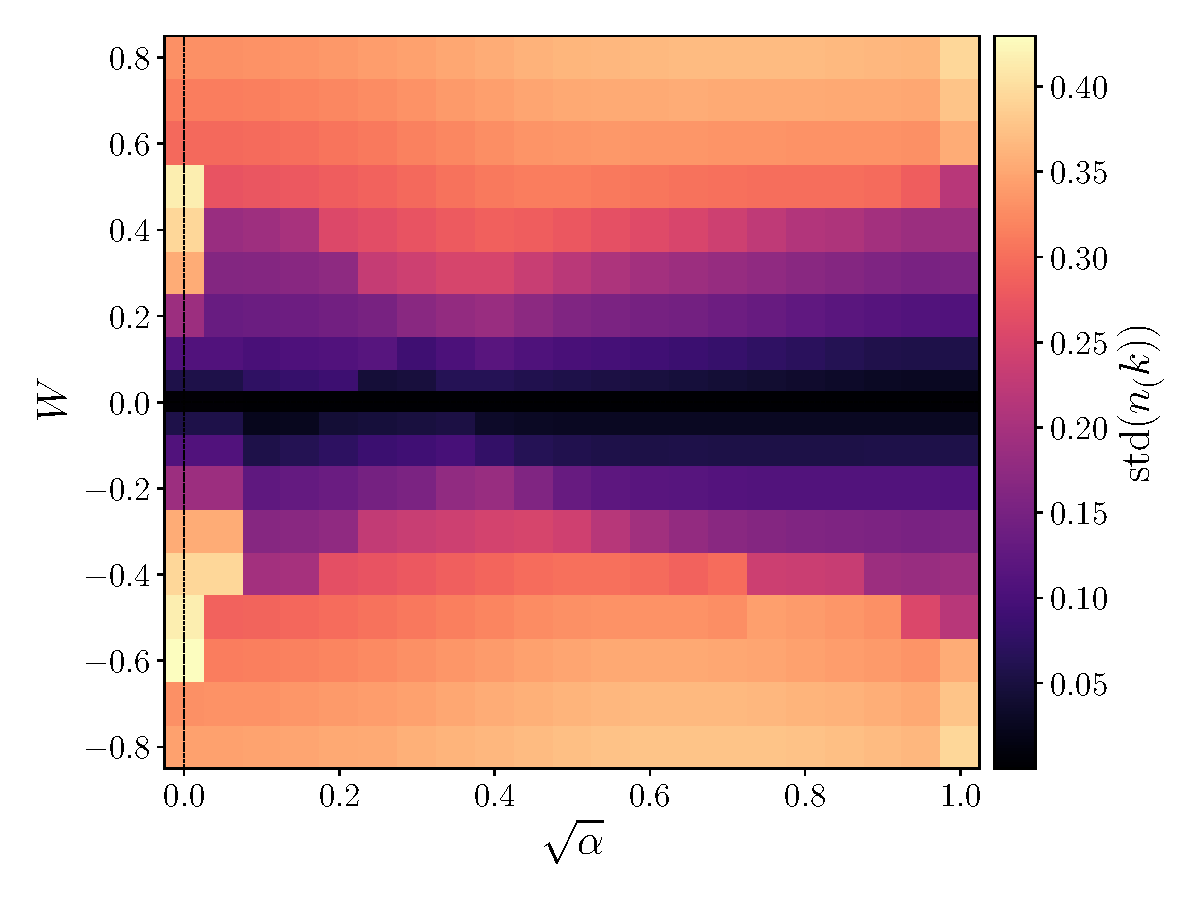
\includegraphics[width=0.5\textwidth]{plots/density_third_third_std_mesh.pdf}
    \caption{Standard deviation of $n(\mathbf{k})$ over the Brillouin zone as a function of $\alpha$ and $W$, at $\nu=\frac{2}{3}$.}\label{fig:third_third_density}
\end{figure}

Figure~\ref{fig:third_third_density} shows that the occupation is essentially flat at $W\approx 0$, while its standard deviation grows large at large $|W|$, confirming the expected Fermi-liquid character of the large-$|W|$ phases. The gapless VP phase likewise shows a non-flat occupation, consistent with Fermi-liquid behavior there. Two additional regions of low standard deviation stand out, surviving up to a discontinuity at relatively large $|W|$. The lower of these regions may correspond to an IVC phase undergoing a Stoner-like transition into a FL state analogous to the case of the depolarizing transition from the VP state, but with a different order parameter. This would agree with Ref.~\cite{raines2024unconventional}, where the VP state is expected to prevail at $\alpha < 0$ and the IVC at $\alpha > 0$, both with phase transitions of the same nature. A schematic summary including these candidate phases is given in Fig.~\ref{fig:summary}.
The larger--$\alpha$ flat occupation region is not studied in detail here.

\subsection{Screening of the interaction}

\begin{figure}[htbp]
    \centering
    \begin{subfigure}{0.45\textwidth}
        \centering
        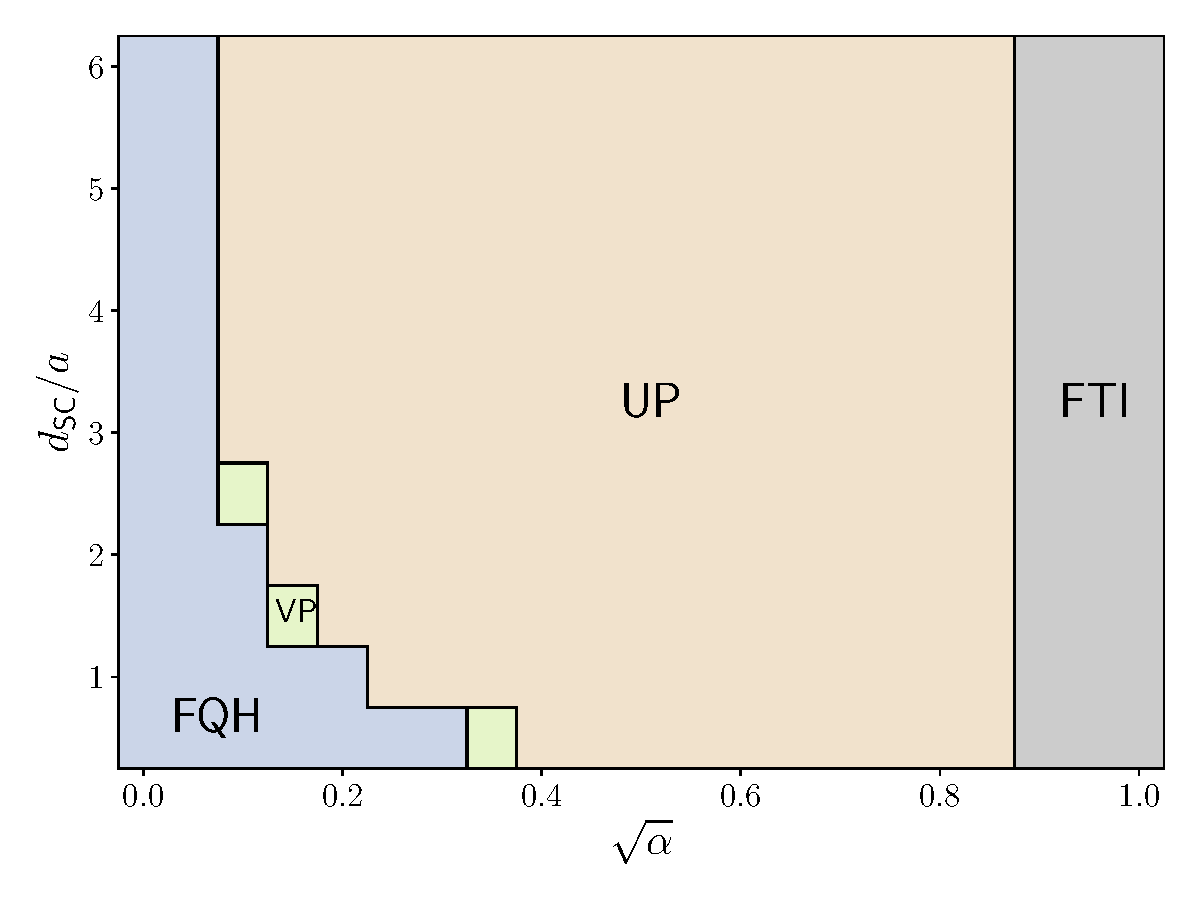
\includegraphics[width=1.0\textwidth]{plots/third_third_screening_alpha_vs_d_phase_diagram.pdf}
        \subcaption{$\alpha$ vs.\ $d_{\text{SC}}/a$, at $l_{\text{RK}} = 0$}\label{fig:third_third_screening_alpha_vs_d_phase_diagram_a}
    \end{subfigure}
    \begin{subfigure}{0.45\textwidth}
        \centering
        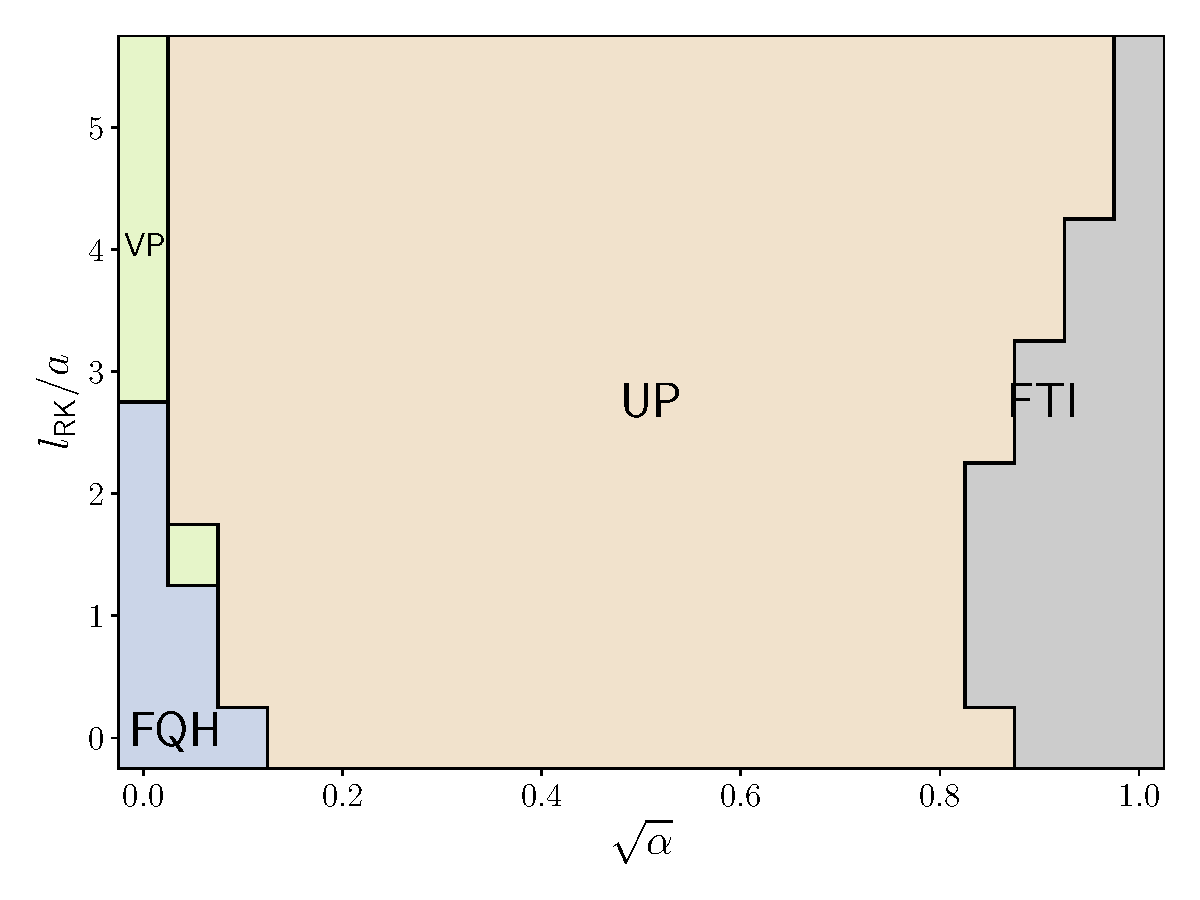
\includegraphics[width=1.0\textwidth]{plots/third_third_screening_alpha_vs_lRK_phase_diagram_d5.01.pdf}
        \subcaption{$\alpha$ vs.\ $l_{\text{RK}}/a$, at $d_{\text{SC}} = 2a$}\label{fig:third_third_screening_alpha_vs_lRK_phase_diagram_b}
    \end{subfigure}
    \caption{Phase diagrams of the $\nu = \frac{2}{3}$ filling at $W=0$ with respect to the screening parameters.}\label{fig:third_third_screening_alpha_vs_d_phase_diagram}
\end{figure}

The stability of the topological phases was tested against the two screening parameters $d_{\text{SC}}$ and $l_{\text{RK}}$. Figure~\ref{fig:third_third_screening_alpha_vs_d_phase_diagram_a} shows the extent of the phases at $W=0$ as a function of $\alpha$ and the screening length $d_{\text{SC}}$. Two conclusions follow. First, the $\alpha$-stability of the FQH phase decreases monotonically with increasing $d_{\text{SC}}$, in agreement with the analytic mean-field estimate, where increasing $d_{\text{SC}}$ shifts the $\alpha_c$ phase boundary in the same direction. Second, no corresponding change in the stability of the FTI phase is visible.

Figure~\ref{fig:third_third_screening_alpha_vs_lRK_phase_diagram_b} shows the analogous dependence on $l_{\text{RK}}$ at $W=0$. Here the stability of both topological phases varies: the FQH phase again becomes less stable with increasing $l_{\text{RK}}$, while the FTI phase instead shows a non-monotonic dependence, with a maximum of stability at finite $l_{\text{RK}}$.

\begin{figure}[htbp]
\centering
\begin{tikzpicture}[
    node distance = 0.6cm and 1.25cm, % Vertical and Horizontal spacing
    arrowstyle/.style={->, >=Stealth, thick, color=ethpetrol},
    labelstyle/.style={font=\small\sffamily, fill=white, inner sep=2pt, rounded corners=1pt, draw=ethpetrol, align=center}
]
    % --- ROW 1 ---
    % Subfigure 1
    \node (sub1) {
        \begin{subfigure}{0.4\textwidth}
            \centering
            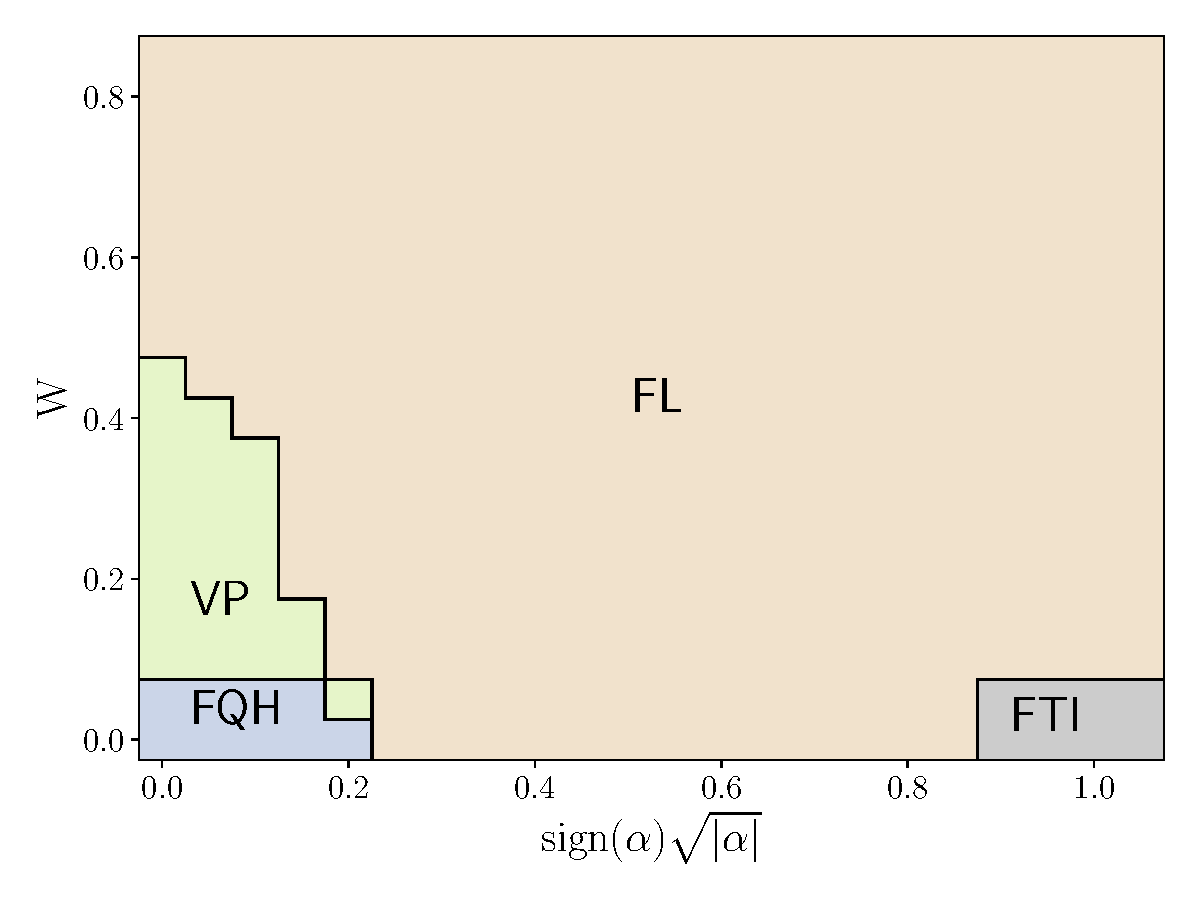
\includegraphics[width=\textwidth]{plots/third_third_screening_alpha_vs_W_phase_diagram_d2.51_lRK0.00.pdf}
            \caption{}
            \label{fig:third_third_screening_alpha_vs_W_phase_diagram_a}
        \end{subfigure}
    };

    % Subfigure 2 (Placed to the right of Subfigure 1)
    \node[right=of sub1] (sub2) {
        \begin{subfigure}{0.4\textwidth}
            \centering
            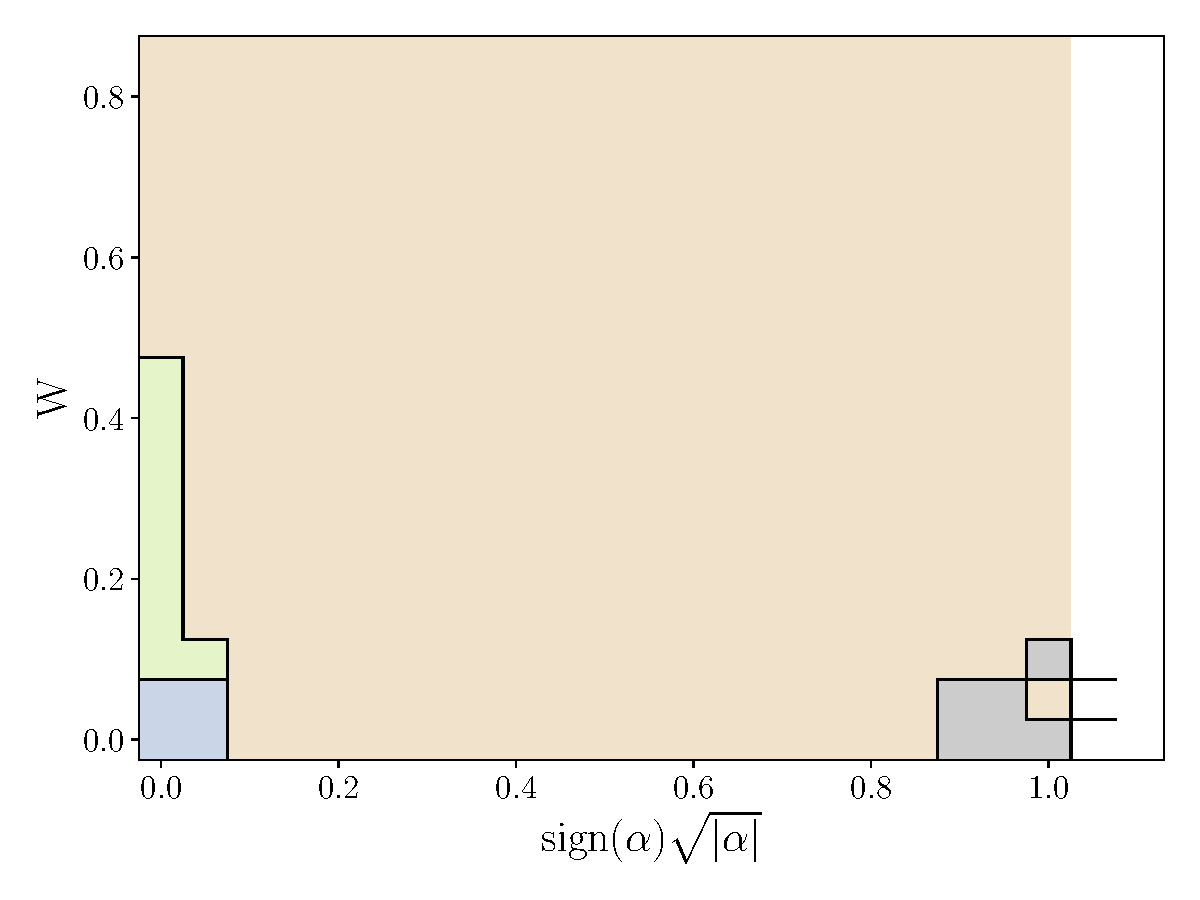
\includegraphics[width=\textwidth]{plots/third_third_screening_alpha_vs_W_phase_diagram_d15.04_lRK0.00.pdf}
            \caption{}
            \label{fig:third_third_screening_alpha_vs_W_phase_diagram_b}
        \end{subfigure}
    };

    % --- ROW 2 ---
    % Subfigure 3 (Centered below the space between sub1 and sub2)
    \node[below=of $(sub1.south)!0.5!(sub2.south)$] (sub3) {
        \begin{subfigure}{0.4\textwidth}
            \centering
            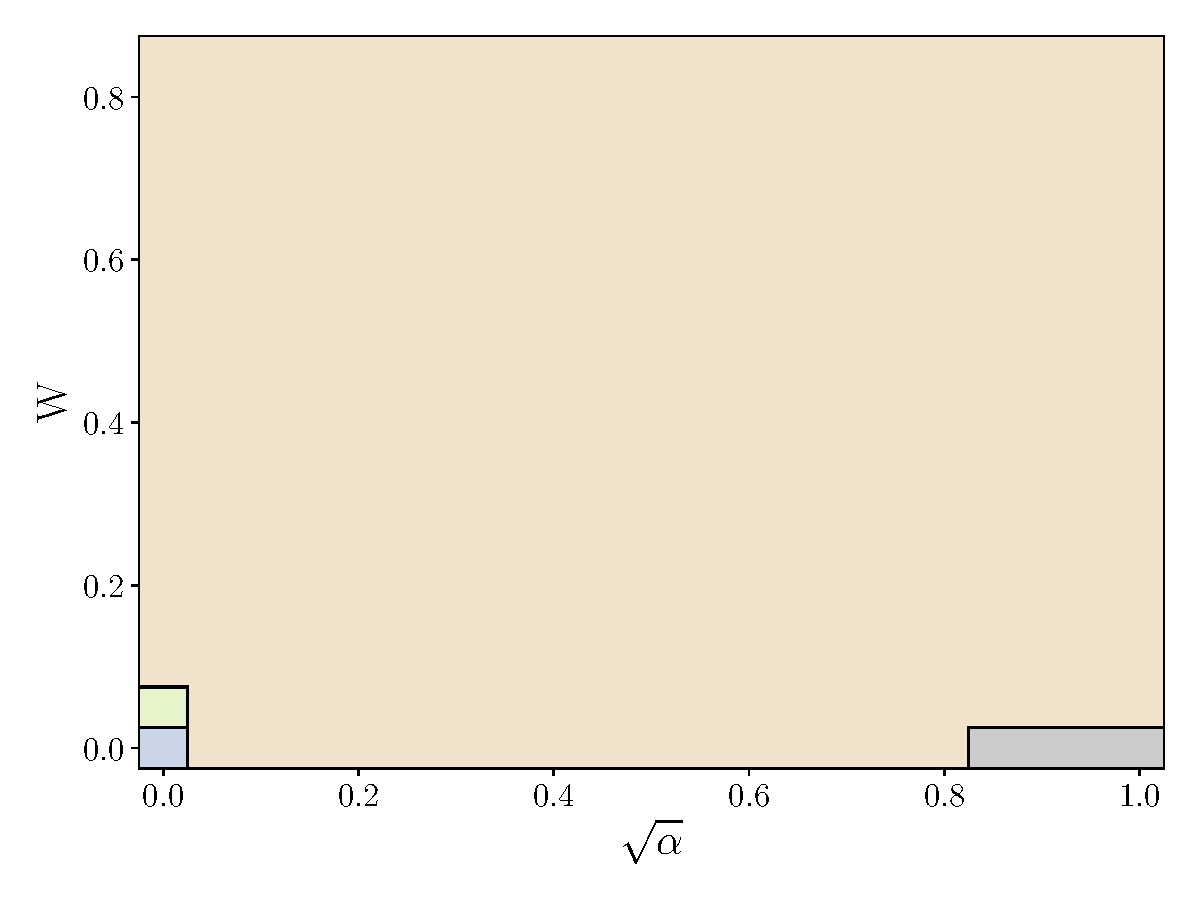
\includegraphics[width=\textwidth]{plots/third_third_screening_alpha_vs_W_phase_diagram_d15.04_lRK5.01.pdf}
            \caption{}
            \label{fig:third_third_screening_alpha_vs_W_phase_diagram_c}
        \end{subfigure}
    };

    % --- ARROWS ---
    % Arrow 1: Plot 1 -> Plot 2
    \draw[arrowstyle] ($(sub1.east) + (-5pt,0)$) -- ($(sub2.west) + (15pt,0)$) 
        node[midway, labelstyle] {$\mathbf{d_{\mathrm{SC}} \nearrow }$};

    % Arrow 2: Plot 2 -> Plot 3 (Connects bottom of Plot 2 to right edge of centered Plot 3)
    \draw[arrowstyle] ($(sub2.south west) + (15pt,30pt)$) -- ($(sub3.north) + (0, -5pt)$)%($(sub2.south west) + (10pt,-5pt)$) -- ($(sub3.north) + (0, 5pt)$) 
        node[midway, labelstyle] {$\mathbf{l_{\mathrm{RK}} \nearrow }$};

\end{tikzpicture}
\caption{Phase diagrams of the $\nu = \frac{2}{3}$ filling in the $\alpha$--$W$ plane with different screening $d_{\text{SC}}$ and $l_{\text{RK}}$. Arrows indicate the direction of change of the parameters.\ (a) $d_{\text{SC}} = 1a$, $l_{\text{RK}} = 0$.\ (b) $d_{\text{SC}} = 6a$, $l_{\text{RK}} = 0$.\ (c) $d_{\text{SC}} = 6a$, $l_{\text{RK}} = 2a$.}\label{fig:third_third_screening_alpha_vs_W_phase_diagram_mindmap}
\end{figure}

Figure~\ref{fig:third_third_screening_alpha_vs_W_phase_diagram_mindmap} shows the full $\alpha$--$W$ phase diagram at different screening parameters, allowing the $W$-stability to be examined alongside the $\alpha$-stability. The main conclusion is that the $W$-stability is essentially independent of $d_{\text{SC}}$, but decreases significantly with increasing $l_{\text{RK}}$. This is particularly relevant for the FTI phase, where seemingly to gain $\alpha$-stability by tuning the screening, one must sacrifice the $W$-stability.

\section{\texorpdfstring{Phase diagram for $\nu = 1$}{Phase diagram for nu = 1/2 + 1/2}}

While fractional topological states are not expected at $\nu=1$ in the LLL, this filling has been studied in the literature and serves as a useful benchmark for the method, as well as a reference point for $n=1$ LL calculations in Chapter~\ref{ch:results_1LL}~\cite{das2025fractional, kwan2025textured}.

\begin{figure}[htbp]
    \centering
    \begin{subfigure}{0.45\textwidth}
        \centering
        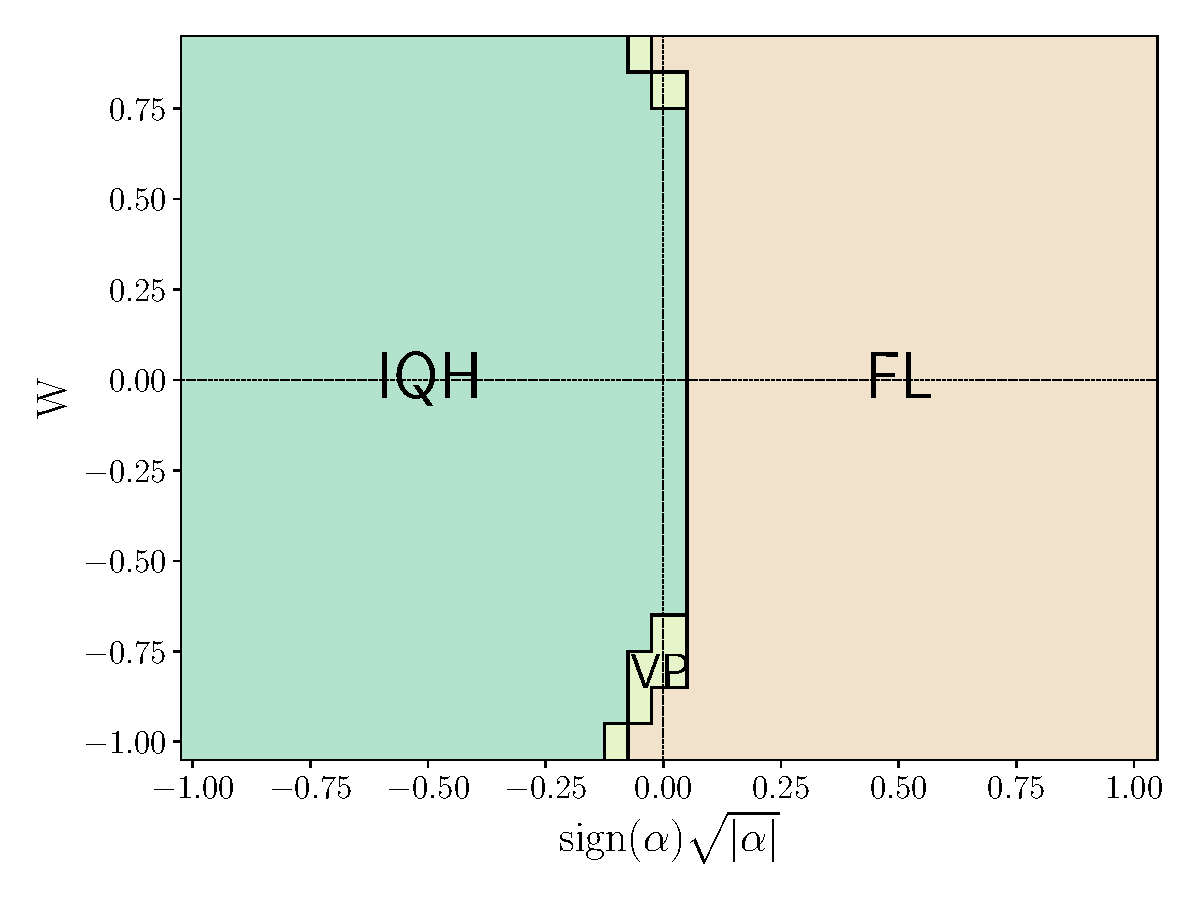
\includegraphics[width=1.0\textwidth]{plots/half_half_phase_diagram.pdf}
        \subcaption{$U(q=0)\neq 0$}\label{fig:half_half_phase_diagram}
    \end{subfigure}
    \begin{subfigure}{0.45\textwidth}
        \centering
        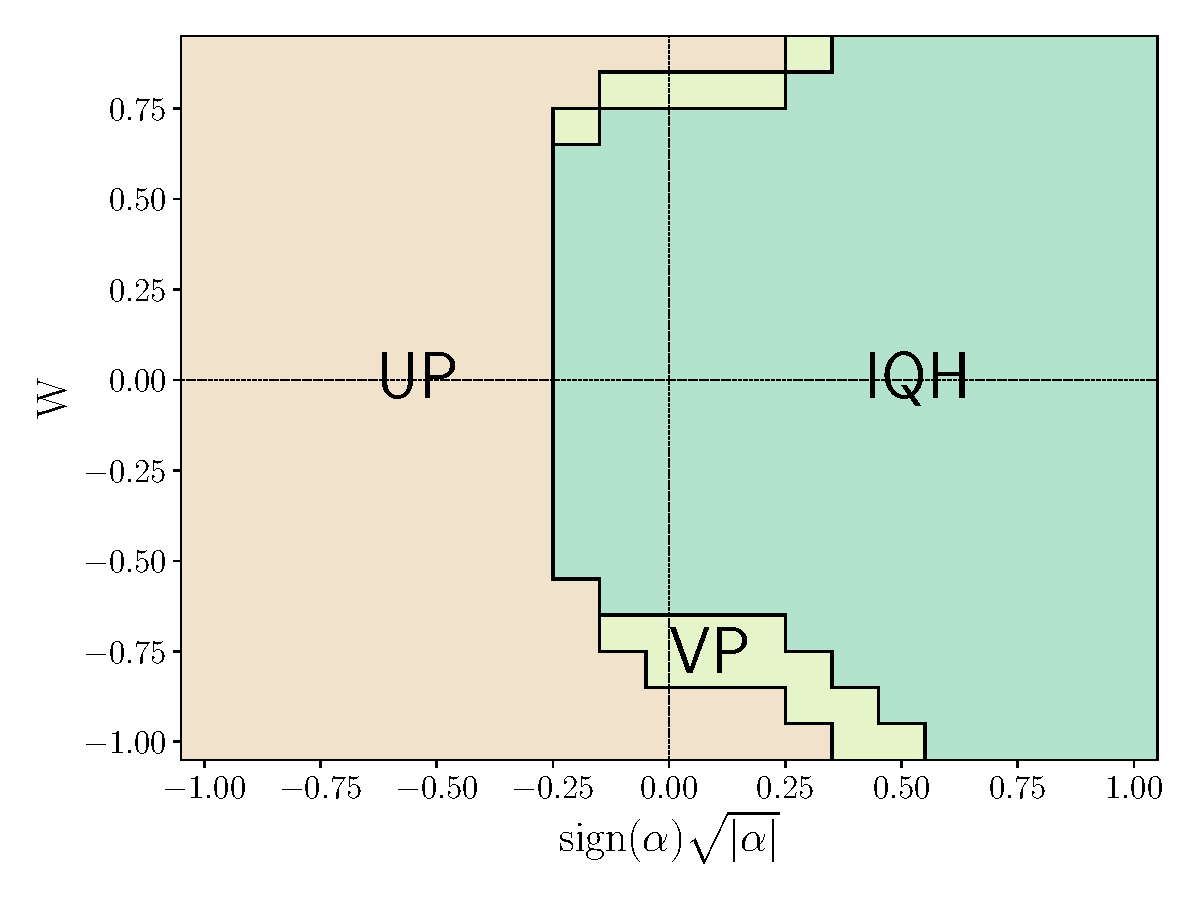
\includegraphics[width=1.0\textwidth]{plots/half_half_q0_phase_diagram.pdf}
        \subcaption{$U(q=0) = 0$}\label{fig:half_half_q0_phase_diagram}
    \end{subfigure}
    \begin{subfigure}{0.45\textwidth}
        \centering
        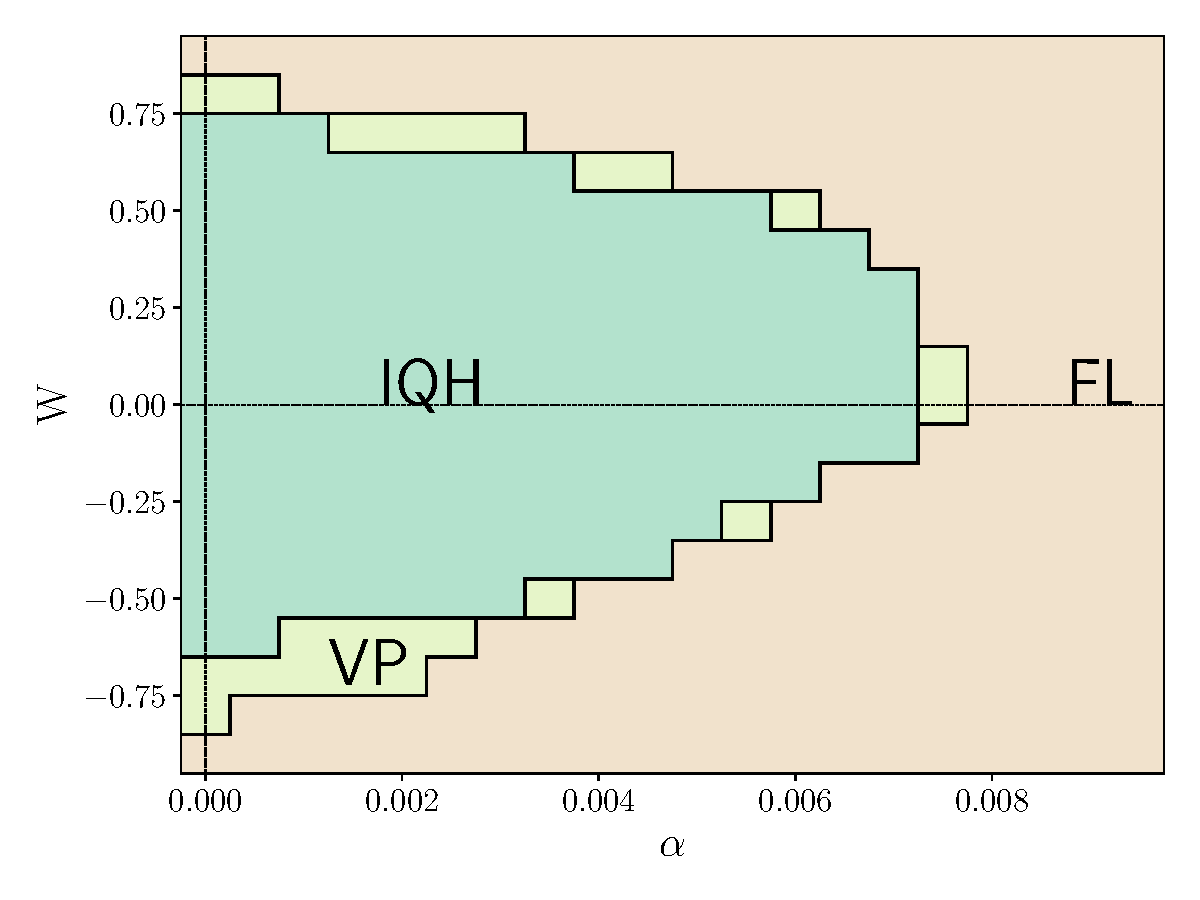
\includegraphics[width=1.0\textwidth]{plots/half_half_zoom_phase_diagram.pdf}
        \subcaption{Zoom-in on the IQH ($U(q=0) \neq 0$)}\label{fig:half_half_zoom_phase_diagram}
    \end{subfigure}
    \begin{subfigure}{0.45\textwidth}
        \centering
        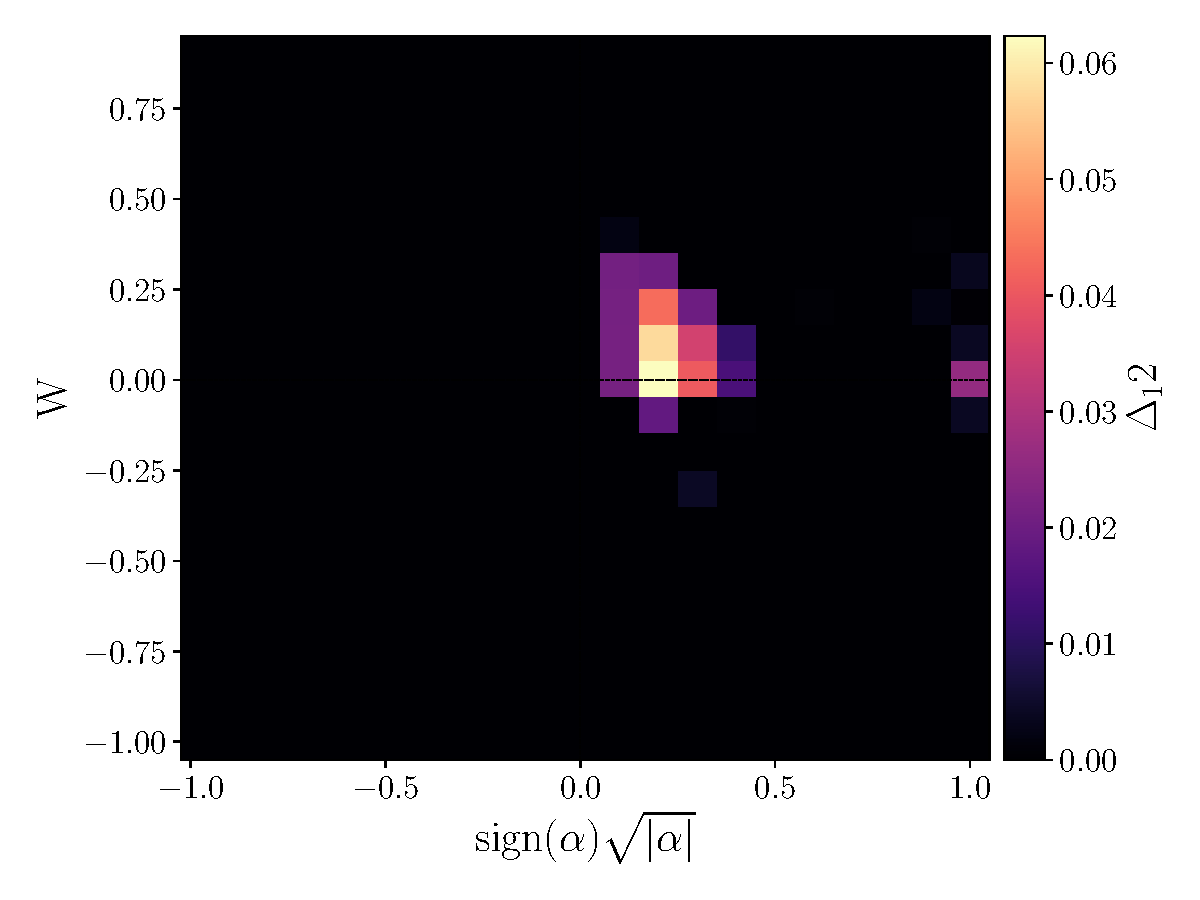
\includegraphics[width=1.0\textwidth]{plots/half_half_gap_n12.pdf}
        \subcaption{$\Delta_{12}$ gap, $U(q=0)\neq 0$}\label{fig:half_half_gap_n12}
    \end{subfigure}
    \caption{Phase diagrams of the $\nu = 1$ filling. UP:\@ general unpolarized state. IQH:\@ valley-polarized integer quantum Hall state. See Fig.~\ref{fig:summary} for a schematic identification of the UP regions.}\label{fig:half_half_phases}
\end{figure}

Figure~\ref{fig:half_half_phases} shows the resulting phase diagram. With $U(\mathbf{q}=0) \neq 0$, similarly to the $\nu=\frac{2}{3}$, a valley-polarized region is found at low $\alpha$, giving way to a gapless non-polarized phase at larger $\alpha$ or larger $|W|$. Due to integer filling, the valley-polarized phase is the IQH state at $\nu = 1 + 0$ and with $\Delta_1 > 0$. The resulting phase boundary is consistent with past results~\cite{kwan2025textured} and with the numerical mean-field estimate, within the same order of magnitude.

The nature of the high--$\alpha$ gapless state can again be discussed in light of the literature and the momentum-occupation function. In the $\alpha = 1$, $W=0$ limit, the $\nu = \tfrac{1}{2} + \tfrac{1}{2}$ state is known to consist of decoupled composite Fermi liquids, $\ket{\text{CFL}} \otimes \overline{\ket{\text{CFL}}}$, while at large bandwidth $|W|$, where kinetic energy dominates, it becomes a pair of Fermi liquids, $\ket{\text{FL}} \otimes \overline{\ket{\text{FL}}}$. The phase transition and boundary between these two states, and the nature of the intermediate states once $\alpha \neq 1$ cannot be resolved with the limited extent of the simulations performed here.

With $U(\mathbf{q}=0) = 0$, the phase diagram shown in Figure~\ref{fig:half_half_q0_phase_diagram} is again inverted. While containing the same phases (IQH, VP and UP) and the same $W$ dependence, now the ground state is unpolarized at low $\alpha$ while the IQH is prevalent at high $\alpha$.

\subsection{\texorpdfstring{Intermediate--$\alpha$ and high-$|W|$ phases}{Intermediate-alpha and high-W phases}}\label{sec:intermediate_alpha_half_half}


\subsubsection{Finite size effects}
Returning to the $U(\mathbf{q}=0)\neq 0$ case, at intermediate $\alpha$, a $\Delta_{12} \neq 0$ gap is found (Fig.~\ref{fig:half_half_gap_n12}), similarly to the $\nu=\tfrac{2}{3}$ system. Such degeneracy does not correspond to any topologically nontrivial state and phase winding is not present. Since the degeneracy is equal to the number of unit cells, it suggests complete translational symmetry breaking in a form of phase separation. It is important to note that the gap is nonzero only for $W \geq 0$, which suggests that the state might stem from finite size effects. An IVC state was reported in this region of the phase diagram by Ref.~\cite{kwan2025textured}, with the peak of the IVC order parameter $\Delta_q$ at $q = \mathbf{Q_0} = (\tfrac{Q}{2},\tfrac{Q}{2})$. The default $3\times 4$ BZ sampling studied here does not contain this point, which might result in favoring other competing phases. To clarify the nature of the state an additional calculation is performed at the same filling, with $N_\phi=10$, in a tilted lattice of Figure~\ref{fig:bz_sampling_10}. This lattice, on the other hand, contains the $\mathbf{Q_0}$ point. The sampling is invariant under the $\mathbf{Q_0}$ shift, and is also more isotropic with $\tfrac{|T_1|}{|T_2|}$ closer to $1$.

\begin{figure}[htbp]
    \centering
    \begin{subfigure}{0.45\textwidth}
        \centering
        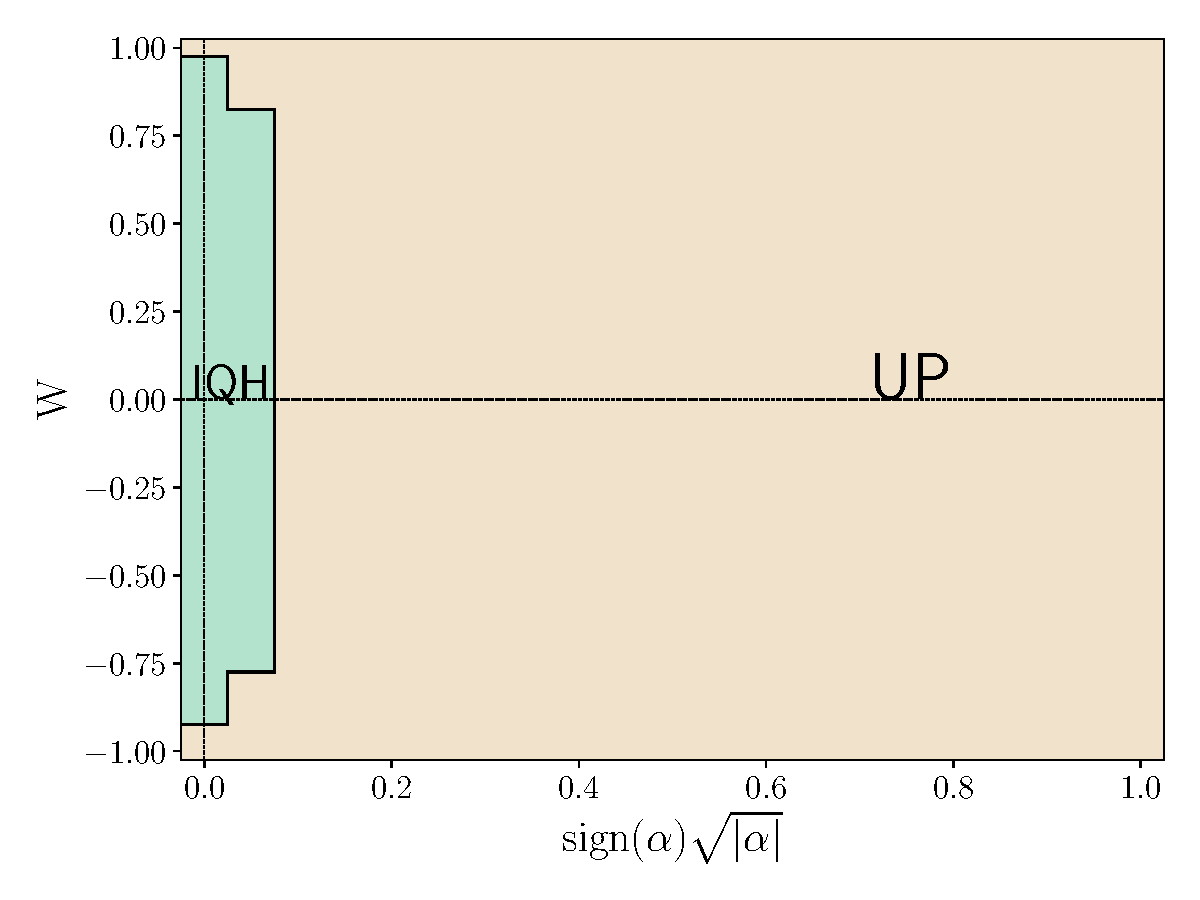
\includegraphics[width=1.0\textwidth]{plots/half_half_tilted_phase_diagram.pdf}
        \subcaption{Phase diagram}\label{fig:half_half_tilted_phase_diagram}
    \end{subfigure}
    \begin{subfigure}{0.45\textwidth}
        \centering
        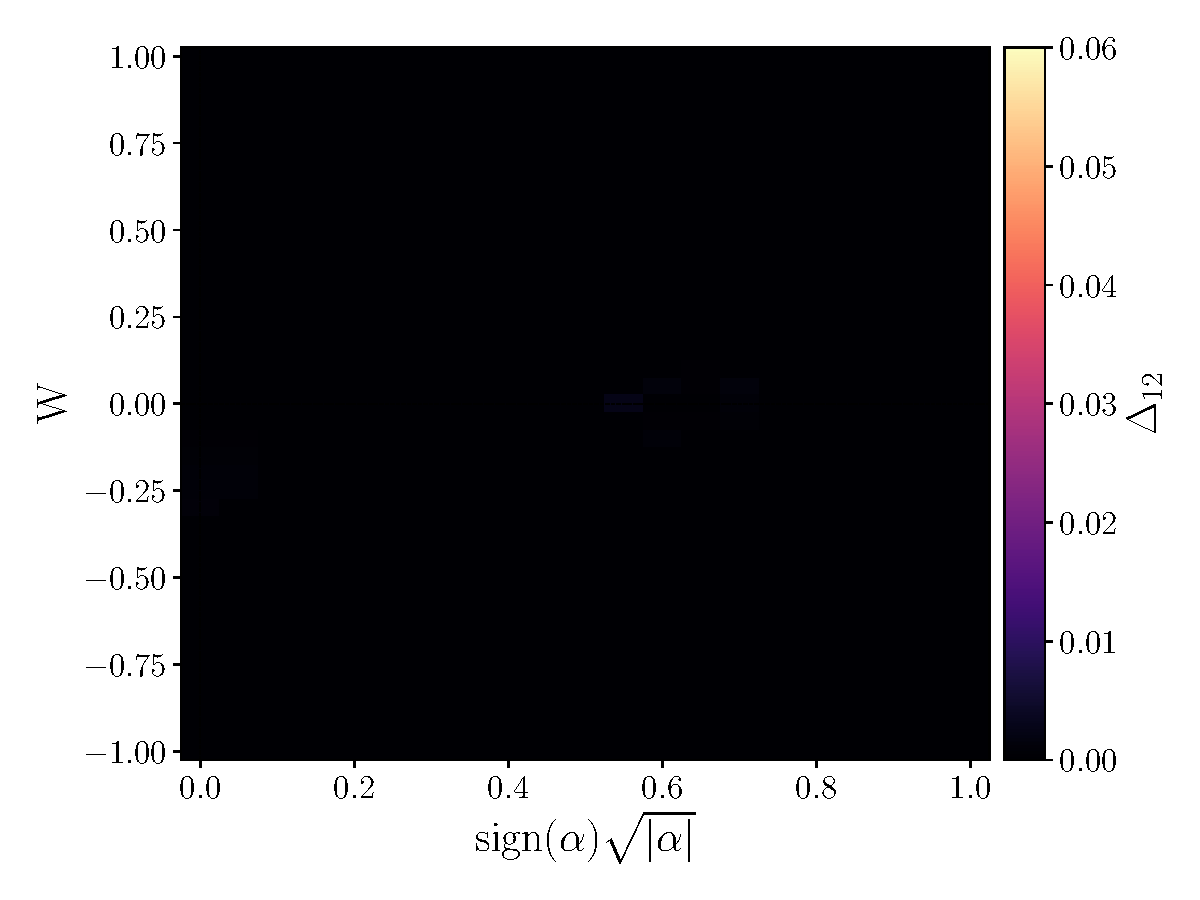
\includegraphics[width=1.0\textwidth]{plots/half_half_tilted_gap_n12.pdf}
        \subcaption{$\Delta_{12}$}\label{fig:half_half_tilted_gap_12}
    \end{subfigure}
    \begin{subfigure}{0.45\textwidth}
        \centering
        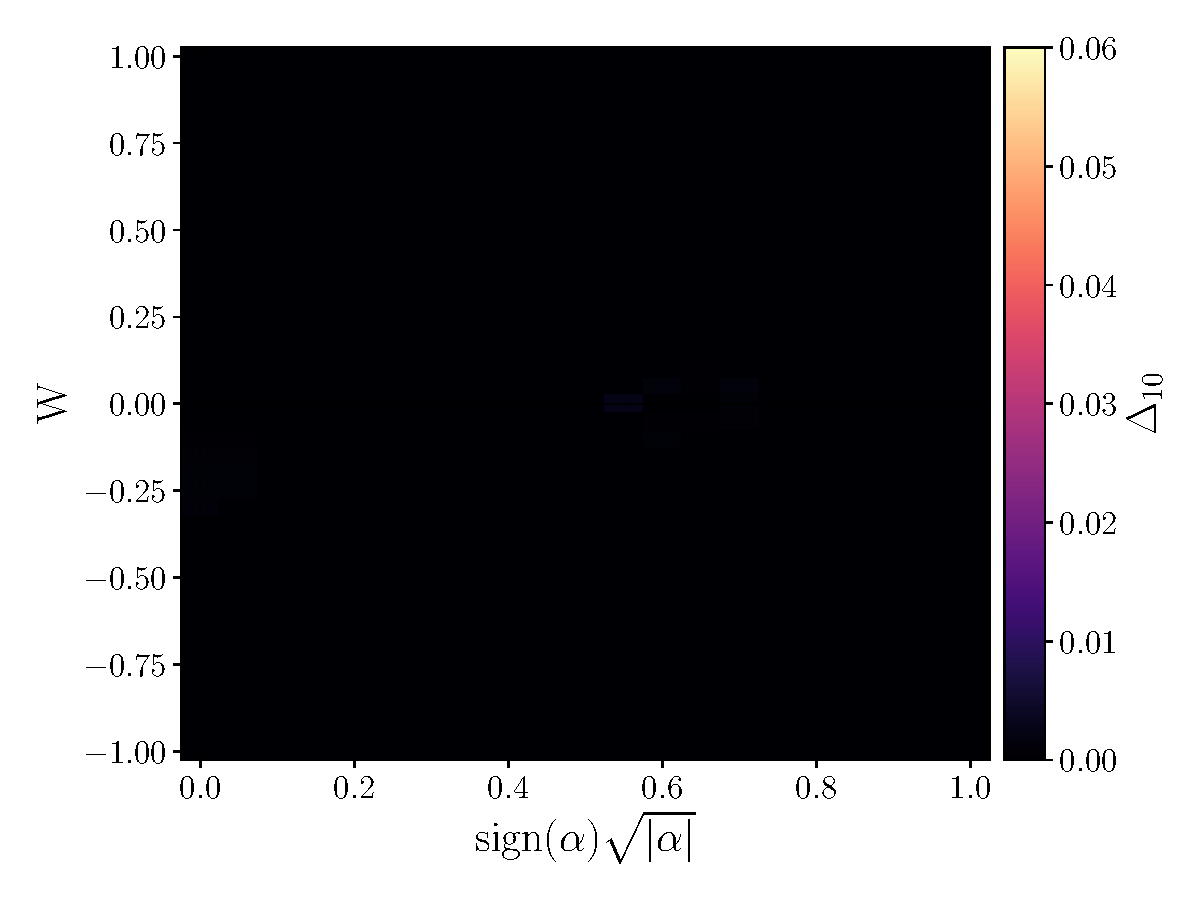
\includegraphics[width=1.0\textwidth]{plots/half_half_tilted_gap_n10.pdf}
        \subcaption{$\Delta_{10}$}\label{fig:half_half_tilted_gap_10}
    \end{subfigure}
    \caption{Phase diagram and gaps in a $\nu=1$ system with tilted boundary conditions of Fig.~\ref{fig:bz_sampling_10}.}\label{fig:half_half_tilted}
\end{figure}

The results are shown in Figure~\ref{fig:half_half_tilted}. First, in this system both the $\Delta_{12}$ gap --- as a comparison with the $3\times 4$ system --- and the $\Delta_{10}$ gap --- corresponding now to the number of unit cells in the system --- are strictly $0$, confirming that the gapped phase is favored only due to finite size effects or anisotropy of the cluster. Second, in Figure~\ref{fig:half_half_tilted_phase_diagram} the phase diagram is perfectly symmetric with respect to $W=0$, confirming the prediction of \S\ref{sec:symmetries} to be exact when the BZ sampling is invariant under the $\mathbf{Q_0}$ shift.


\subsubsection{Momentum-occupation function}
\begin{figure}[htbp]
    \centering
    \begin{subfigure}{0.45\textwidth}
        \centering
        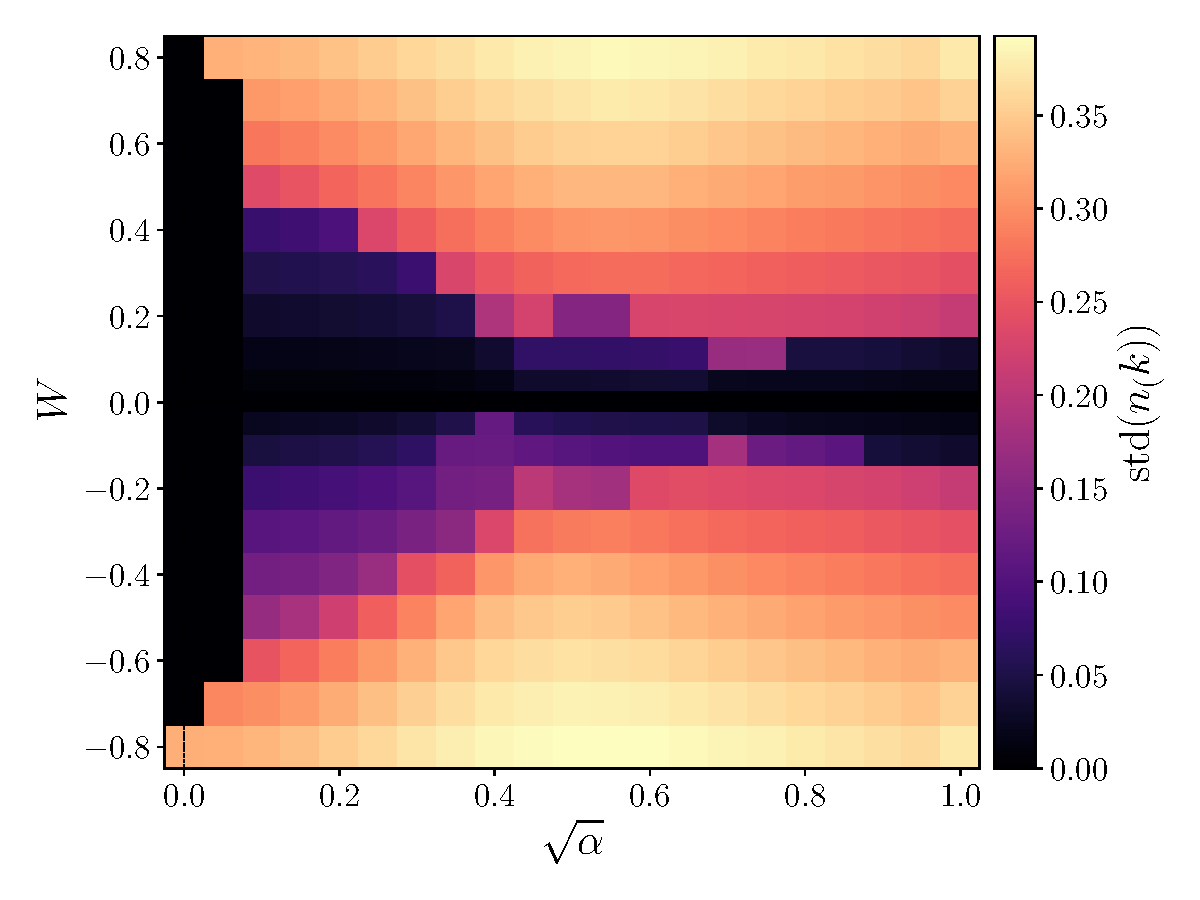
\includegraphics[width=1.0\textwidth]{plots/density_half_half_std_mesh.pdf}
        \subcaption{Standard deviation of $n(\mathbf{k})$ vs.\ $\alpha$, $W$}\label{fig:half_half_density_std}
    \end{subfigure}
    \begin{subfigure}{0.45\textwidth}
        \centering
        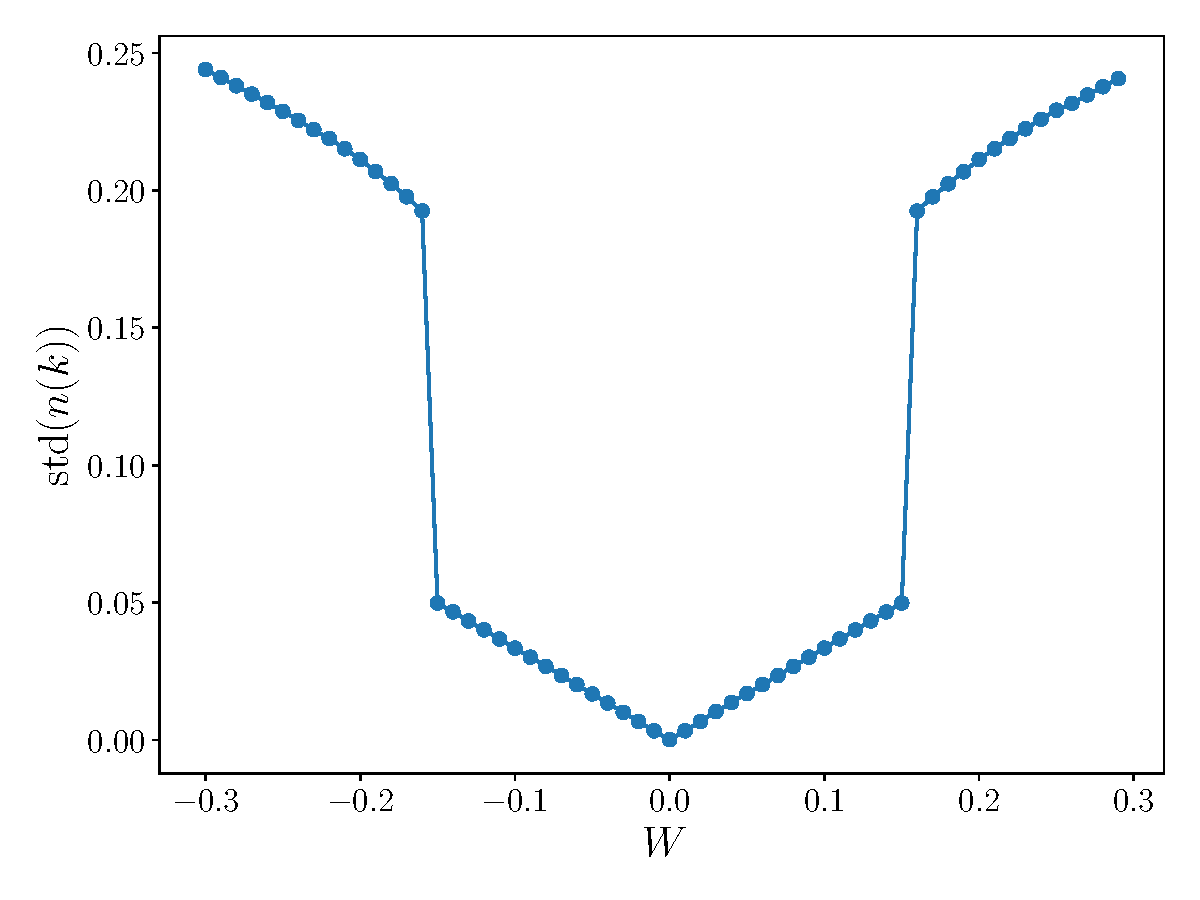
\includegraphics[width=1.0\textwidth]{plots/density_half_half_alpha1_std_cut_alpha_1.00.pdf}
        \subcaption{Cut of (a) at $\alpha=1$}\label{fig:half_half_density_cut}
    \end{subfigure}
    \begin{subfigure}{0.45\textwidth}
        \centering
        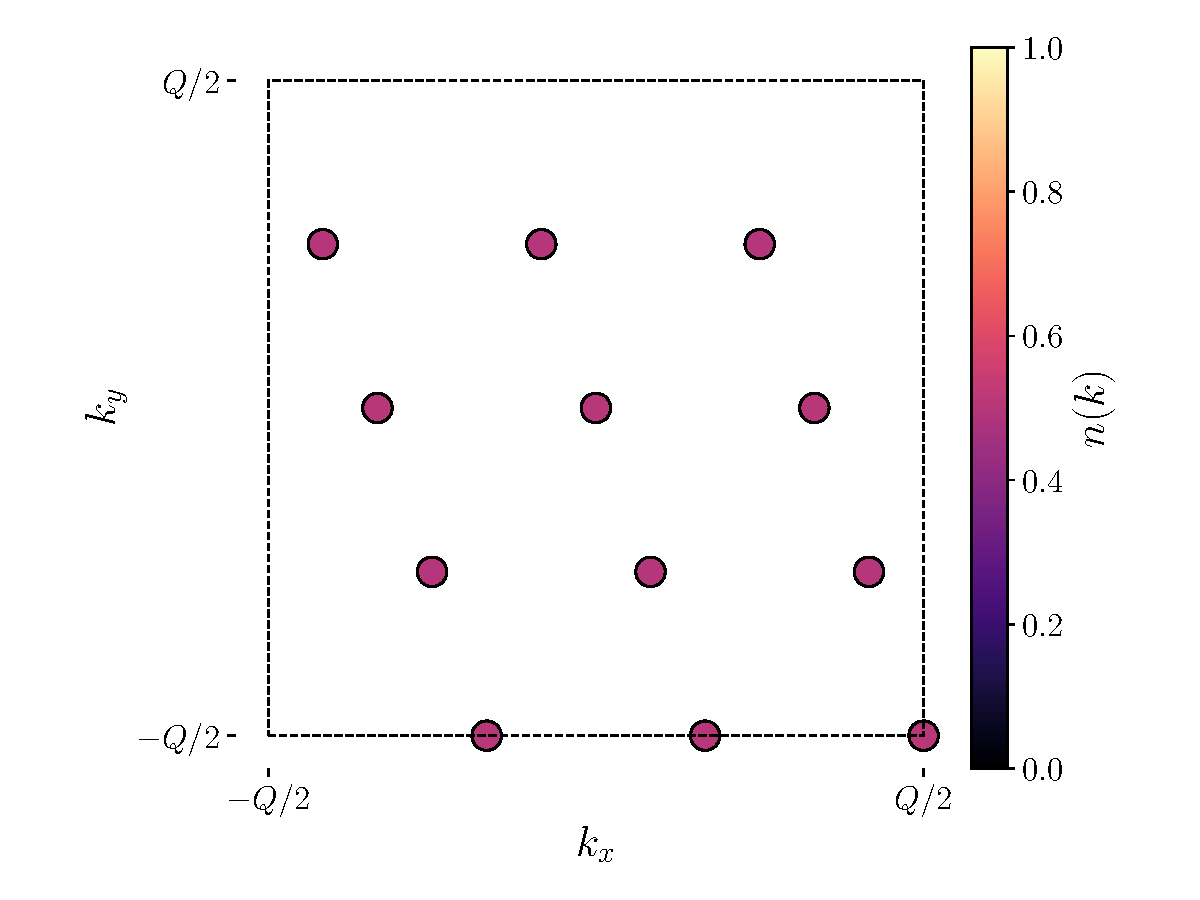
\includegraphics[width=1.0\textwidth]{plots/density_half_half_nk_W_0.00_alpha_1.00.pdf}
        \subcaption{$n(\mathbf{k})$ at $W=0.0$, $\alpha=1.0$\\ $\ket{\text{CFL}} \otimes \overline{\ket{\text{CFL}}}$}\label{fig:half_half_density_CFL}
    \end{subfigure}
    \begin{subfigure}{0.45\textwidth}
        \centering
        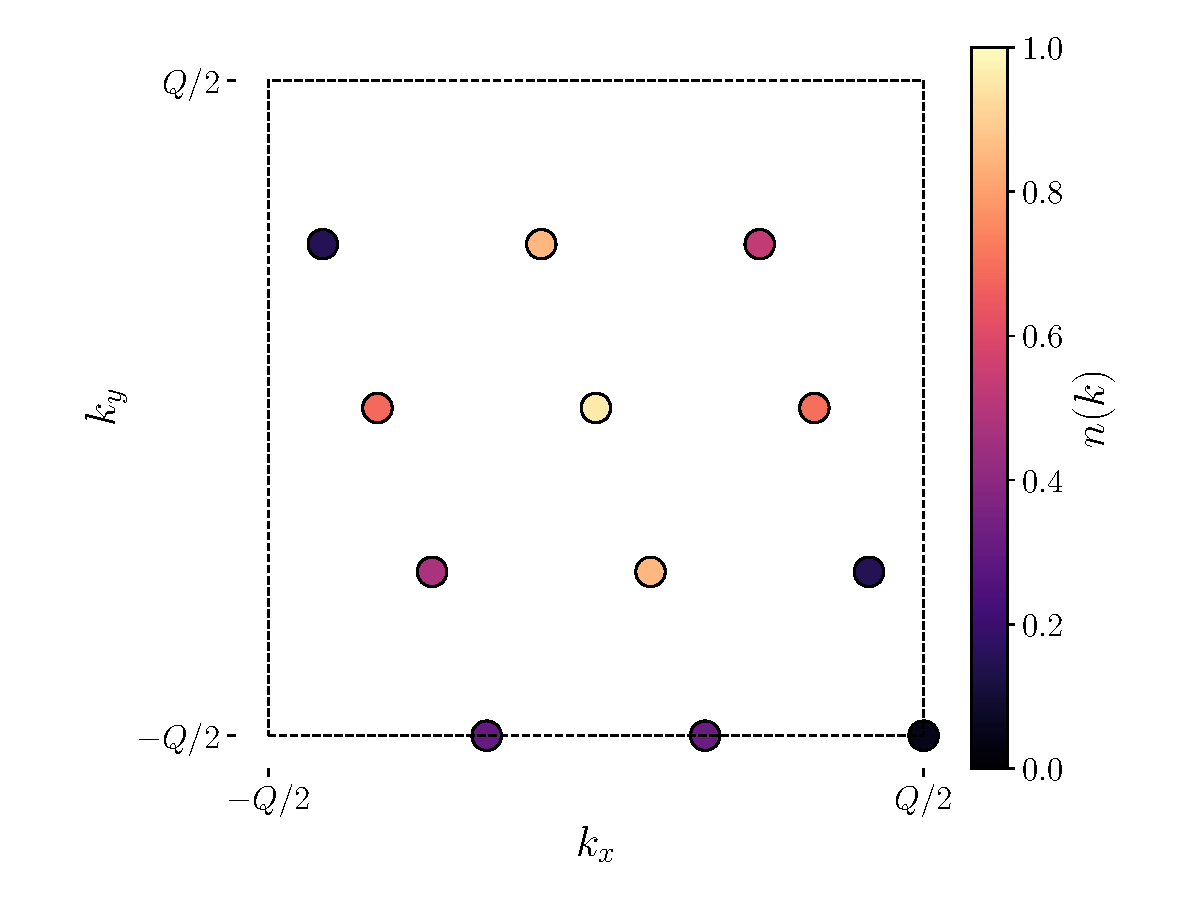
\includegraphics[width=1.0\textwidth]{plots/density_half_half_nk_W_0.50_alpha_1.00.pdf}
        \subcaption{$n(\mathbf{k})$ at $W=0.5$, $\alpha=1.0$\\ $\ket{\text{FL}} \otimes \overline{\ket{\text{FL}}}$}\label{fig:half_half_density_FL}
    \end{subfigure}
    \caption{The momentum-space occupation $n(\mathbf{k})$ for the $\nu=1$ filling, shown for an arbitrary valley.}\label{fig:half_half_density}
\end{figure}

Figure~\ref{fig:half_half_density} shows the standard deviation of $n(\mathbf{k})$ over the Brillouin zone. A large region of flat occupation is again observed at $\sqrt{\alpha} \in [0.05, 0.4]$, which, by comparison with the literature, may correspond to the IVC state, with a discontinuous transition to the Fermi liquid at higher $|W|$: while Kwan et al.~\cite{kwan2025textured} confirm the IVC phase, the transition itself is not reported there --- IVC being also found at higher $W$. The same discontinuity of $n(\mathbf{k})$ is found both at $W > 0$ and at $W < 0$ in both the default and the tilted cluster calculations, confirming that it is not caused by the phase-separated state found only in one of these four cases.

The IVC phase reported in Ref.~\cite{kwan2025textured} is a gapped Chern-texture insulator, while the state found here is consistently gapless. This is not incompatible with their result, since their Hartree--Fock gap is a charge gap, whereas the gap calculated here is a neutral gap, which is expected to be gapless in the IVC phase due to its Goldstone mode.


Additionally, a clear transition between $\ket{\text{CFL}} \otimes \overline{\ket{\text{CFL}}}$ and $\ket{\text{FL}} \otimes \overline{\ket{\text{FL}}}$ is seen at $\alpha=1$, with a jump in the standard deviation of $n(\mathbf{k})$ at $W \approx 0.17$ (Fig.~\ref{fig:half_half_density_cut}); an analogous transition for a single Landau level was studied by Barkeshli and McGreevy~\cite{barkeshli2012continuous}. The momentum-occupation function is shown explicitly on either side of this transition: it is flat at low $|W|$ (Fig.~\ref{fig:half_half_density_CFL}), and shows a clear Fermi surface at high $|W|$ (Fig.~\ref{fig:half_half_density_FL}).

\section{\texorpdfstring{Phase diagram for $\nu = \frac12$}{Phase diagram for nu = 1/2}}

For completeness, the $\nu = \tfrac{1}{2}$ filling was studied in an analogous way. No gapped topological order is expected here in the lowest Landau level, but the valley polarization is expected to behave qualitatively similarly to the other fillings considered above.

\begin{figure}[htbp]
    \centering
    \begin{subfigure}{0.45\textwidth}
        \centering
        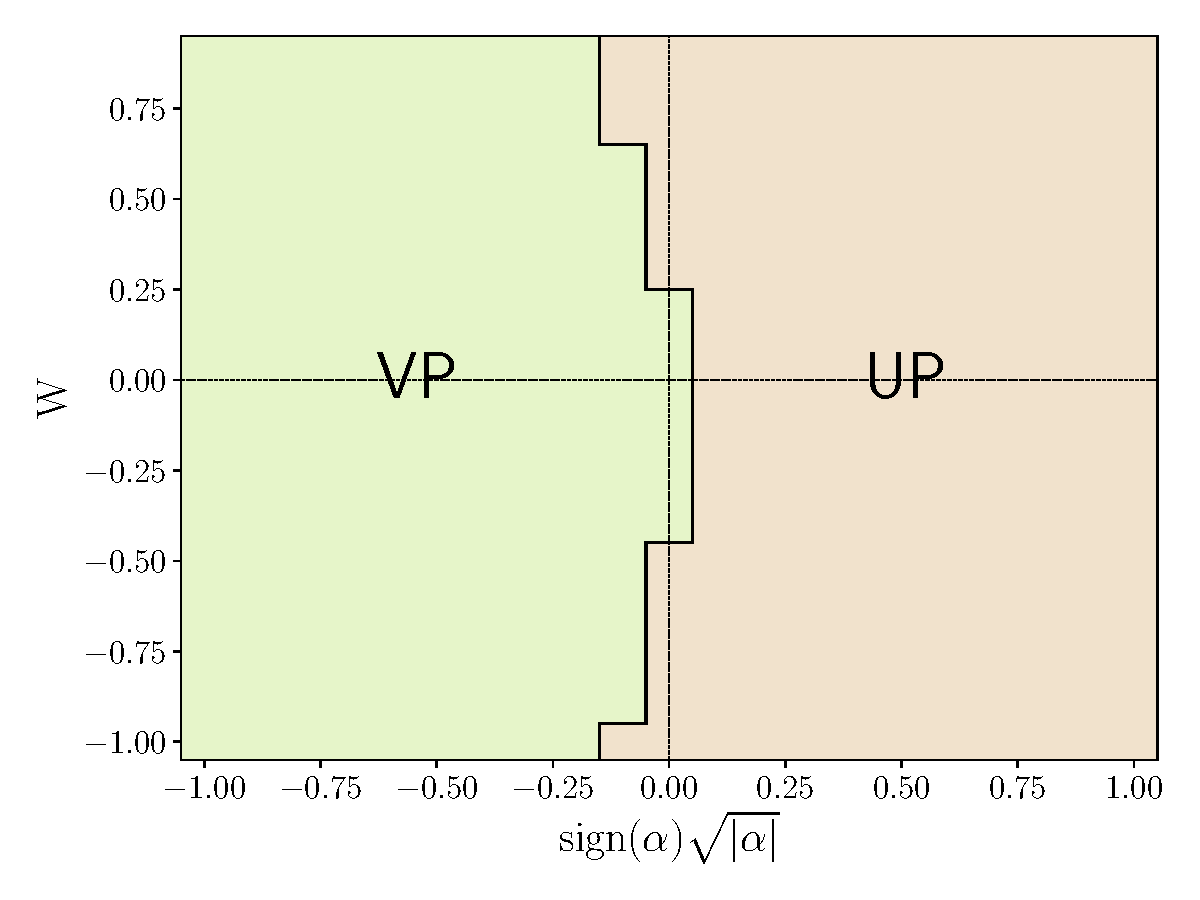
\includegraphics[width=1.0\textwidth]{plots/fourth_fourth_phase_diagram.pdf}
        \subcaption{$U(\mathbf{q}=0)\neq0$}\label{fig:fourth_fourth_phase_diagram}
    \end{subfigure}
    \begin{subfigure}{0.45\textwidth}
        \centering
        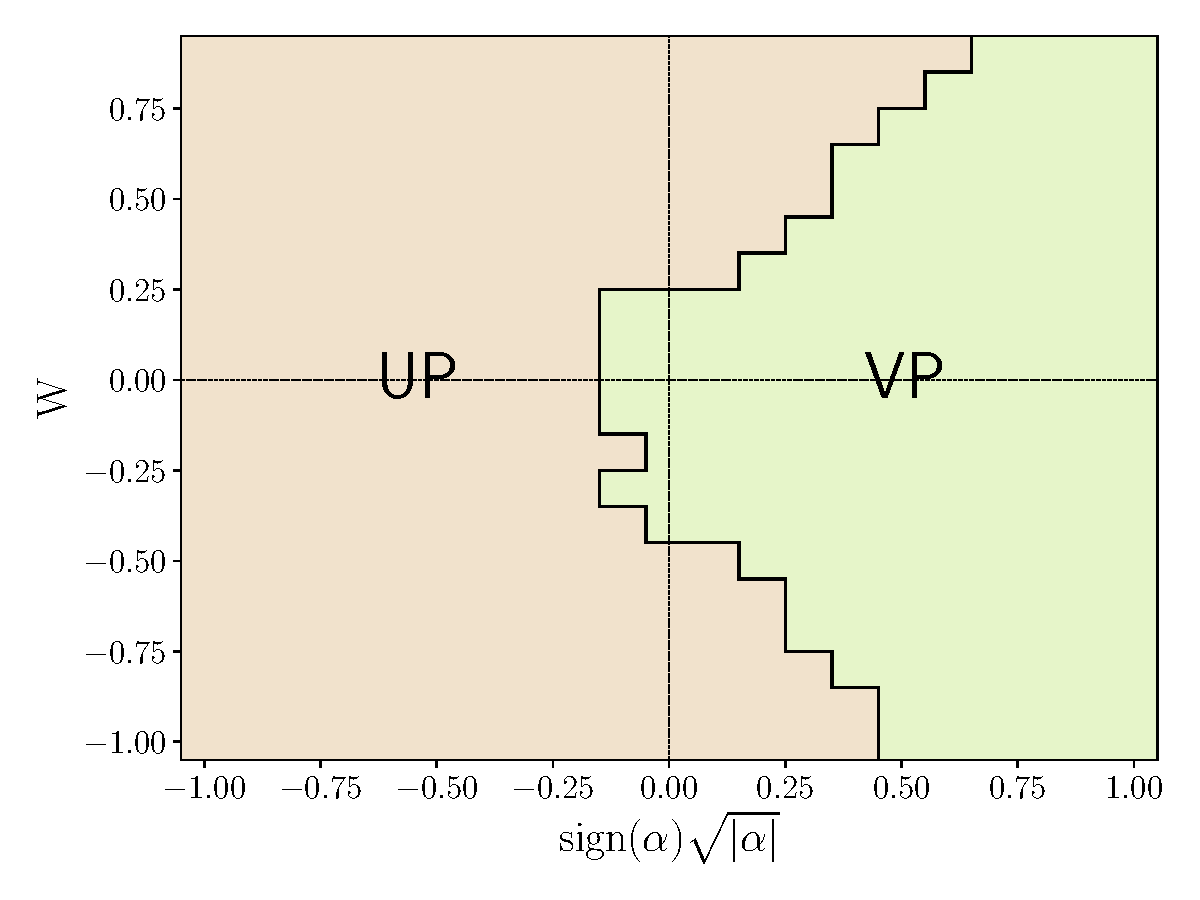
\includegraphics[width=1.0\textwidth]{plots/fourth_fourth_q0_phase_diagram.pdf}
        \subcaption{$U(\mathbf{q}=0) = 0$}\label{fig:fourth_fourth_q0_phase_diagram}
    \end{subfigure}
    \caption{Phase diagrams of the $\nu = \frac{1}{2}$ filling. VP:\@ gapless valley-polarized state. UP:\@ general unpolarized state. See Fig.~\ref{fig:summary} for a schematic identification of the VP/UP regions.}\label{fig:fourth_fourth_phases}
\end{figure}



Figure~\ref{fig:fourth_fourth_phases} shows the resulting phase diagram. With $U(\mathbf{q}=0)\neq 0$, two gapless phases are present: a VP phase at low $\alpha$ or low $|W|$, and a non-polarized phase otherwise. Following the same reasoning as for $\nu=1$, the $\alpha=1$, $W=0$ limit is expected to host a $\ket{\text{CFL}} \otimes \overline{\ket{\text{CFL}}}$ state at $\nu=\tfrac{1}{4} + \tfrac{1}{4}$, while the gapless phase at $\alpha=1$ and high $|W|$ is expected to be $\ket{\text{FL}} \otimes \overline{\ket{\text{FL}}}$; the intermediate parameter regime is harder to characterize unambiguously.

Unlike at the other fillings, the VP state here is similar in nature to the unpolarized state. At $W=0$, the fully valley-polarized system is a $\text{CFL}_{\text{pol.}}$ for all relevant $\alpha$, since with only one valley occupied the inter-valley coupling plays no role; a Stoner-like transition from the valley-polarized to the unpolarized state is again found at large $|W|$. Once again, the phase diagram is approximately symmetric around the $W=0$ axis.

For the $U(\mathbf{q}=0) = 0$ (Figure~\ref{fig:fourth_fourth_q0_phase_diagram}) the same phases are again detected but with the unpolarized region at low $\alpha$ instead of large $\alpha$. The same Stoner-like transition is found at high $|W|$.

\subsection{\texorpdfstring{Momentum-occupation function}{Momentum-occupation function}}
\begin{figure}[htbp]
    \centering
    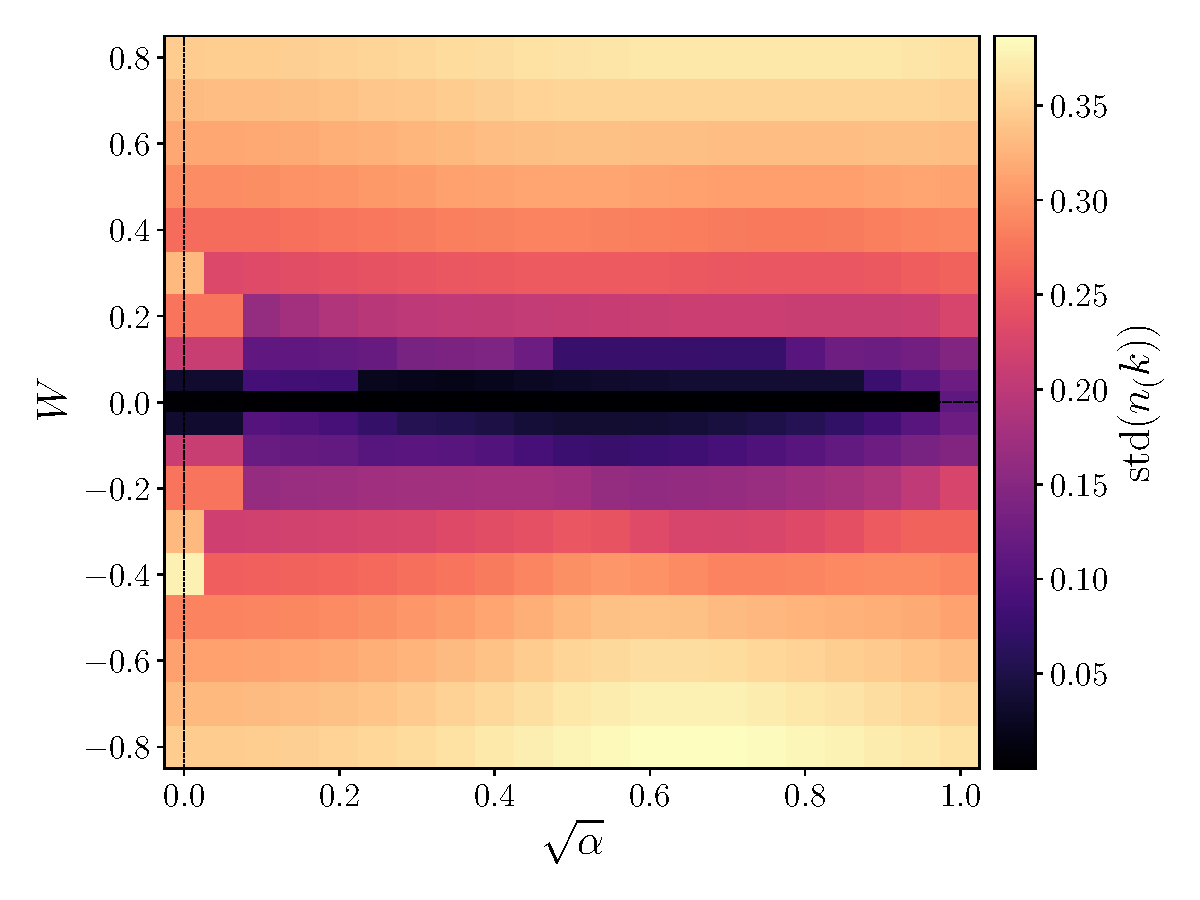
\includegraphics[width=0.5\textwidth]{plots/density_fourth_fourth_std_mesh.pdf}
    \caption{Standard deviation of $n(\mathbf{k})$ over the Brillouin zone as a function of $\alpha$ and $W$, at $\nu=\frac{1}{2}$.}\label{fig:fourth_fourth_density}
\end{figure}

As a further diagnostic for the phases in $U(\mathbf{q} = 0) \neq 0$ case, Fig.~\ref{fig:fourth_fourth_density} shows the standard deviation of $n(\mathbf{k})$ over the Brillouin zone: the occupation is flat at low $|W|$ and develops a clear Fermi surface at high $|W|$. Even though the valley-polarized region is gapless throughout, a clear distinction remains within it between the flat occupation characteristic of a CFL at low $|W|$ and the peaked Fermi surface of an FL at intermediate $|W|$. While not studied in further detail here, a phase transition analogous to the one found at $\nu=1$ is suspected between these states as well.


